\renewcommand{\nomducours}{\nomcourssix}
\renewcommand{\chapterlabel}{chap_six}
\renewcommand{\sousnomducours}{\sousnomcourssix}
\renewcommand{\contentsummaryducours}{\contentsummarycourssix}

\chapter{\nomducours}
\thispagestyle{empty}
\label{\chapterlabel}

\begin{tetedechapitre}[\contentsummaryducours]
	../../contenu/6/contenuintrocours6.tex\par
\end{tetedechapitre}

\section{Conventions graphiques}
\label{ch_conventions_graphiques}

	Nous commençons par nous accorder sur quelques conventions graphiques et de notation, qui sont résumées en \cref{fig_conventions_graphiques_travail_net}.
	
	\begin{figure}
		\begin{center}
			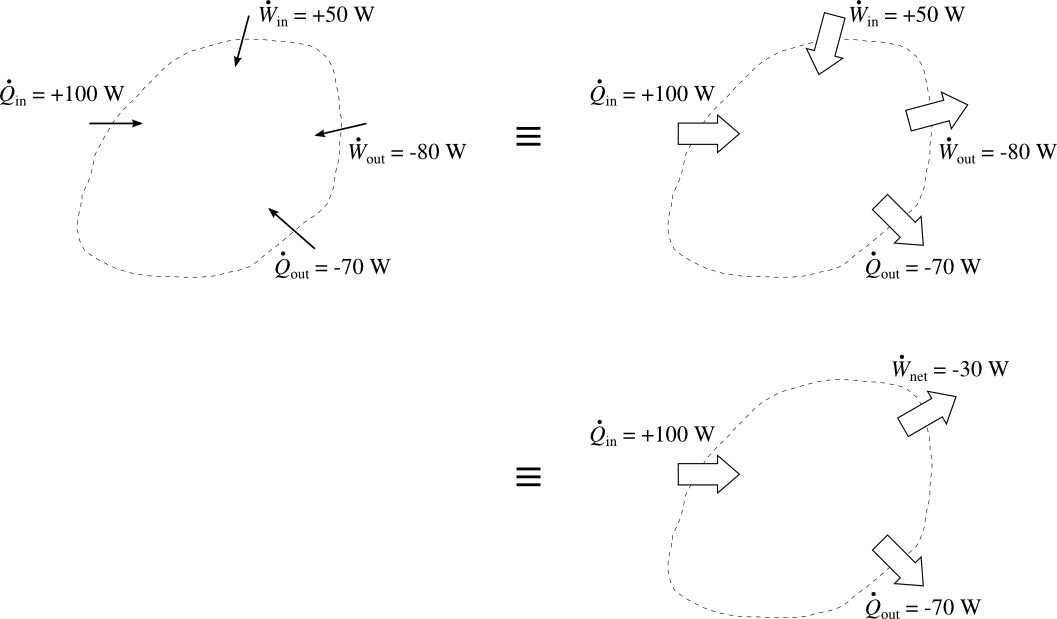
\includegraphics[width=\textwidth]{images/conventions_graphiques_travail_net.png}
		\end{center}
		\supercaption{Nouvelles conventions graphiques et de notation des transferts énergétiques.
			Les flèches blanches sont orientées selon le sens physique des transferts ; La somme algébrique de tous les travaux est représentée par un unique transfert nommé \vocab{travail net}.}{schéma \cczero \oc}
		\label{fig_conventions_graphiques_travail_net}
	\end{figure}

	Nous utilisons de larges flèches blanches pour représenter \emph{le sens physique des transferts}. Nous ne modifions pas notre convention de signe (les transferts sont positifs vers le système et négatifs lorsqu’ils en proviennent), mais seulement la convention graphique pour les orienter, afin de rendre la visualisation des transferts dans les machines plus intuitive.

	La somme algébrique du travail reçu $W_\inn$ et fourni $W_\out$ par une machine est nommé le \vocab{travail net} $W_\net$. Le travail net peut être positif (reçu par la machine de l’extérieur) ou négatif (fourni par la machine à l’extérieur), selon le type d’application.
	\begin{IEEEeqnarray}{rCl}
		W_\net 			& \equiv & W_\inn + W_\out 					\nonumber \\
		\dot W_\net 	& \equiv & \dot W_\inn + \dot W_\out 	\nonumber \\
		w_\net 			& \equiv & w_\inn + w_\out
	\label{def_travail_net}
	\end{IEEEeqnarray}

	On définit la \vocab{chaleur nette} de la même façon :
	\begin{IEEEeqnarray}{rCl}
		Q_\net 			& \equiv & Q_\inn + Q_\out	 				\nonumber \\
		\dot Q_\net 	& \equiv & \dot Q_\inn + \dot Q_\out	\nonumber \\
		q_\net 			& \equiv & q_\inn + q_\out
	\end{IEEEeqnarray}

	Ainsi, par exemple, un moteur automobile reçoit une chaleur nette positive et produit un travail net négatif.


\section{Transformer chaleur et travail}

	\subsection{Construire des cycles thermodynamiques}
	\label{ch_construction_cycle}

		Nous souhaitons comparer différentes manières de transformer travail et chaleur. Pour que ces comparaisons soient valables, il faut que nous tenions toujours compte de \emph{toutes} les transformations subies par le fluide jusqu’à ce qu’il soit revenu à son état initial.

		Par exemple, il est aisé de refroidir une pièce avec une bouteille d’air comprimé (il suffit de faire travailler le fluide pendant sa détente pour que sa température chute) ; mais si nous voulons refroidir la pièce en continu, alors il nous faut aussi tenir compte de l’énergie nécessaire pour \emph{ramener} l’air dans la bouteille, à sa pression et température initiales, à la fin du processus.
		
		Un second exemple est celui d’un moteur automobile, qui rejette de la chaleur emportée par les gaz d’échappement. Pour tenir compte de cette énergie perdue, nous comptabilisons la chaleur qu’il faudrait prélever aux gaz pour les ramener à la température d’entrée du moteur. Ce refroidissement imaginaire a lieu en dehors du moteur en pratique, mais d’un point de vue thermodynamique, il fait partie intégrante du processus de transformation énergétique.

		Ainsi, à chaque fois que nous allons analyser le fonctionnement d’une machine thermique, nous allons prendre soin de poursuivre l’évolution du fluide jusqu’à le ramener à son état initial (même température, même pression, même énergie interne, etc.). Nous disons alors qu’il a parcouru un \vocab{cycle thermodynamique} (\S\ref{ch_premier_principe_sf}).


	\subsection{Produire un travail à partir de chaleur}
	\label{ch_principe_fonctionnement_moteur}

		Commençons par comprimer un fluide : nous augmentons sa pression et réduisons son volume spécifique, ce qui nous demande un certain travail. Après cela, chauffons ce fluide : sa pression et son volume ont tendance à augmenter. En détendant le fluide jusqu’à sa pression initiale, nous allons récupérer un travail plus grand que celui que nous avons investi à l’aller. Pour pouvoir enfin ramener le fluide à son état initial, il faut le refroidir.

		Au final, le fluide a dépensé moins de travail au chemin retour qu’il n’en a reçu à l’aller. Sur un cycle, il aura donc \emph{produit} du travail et absorbé (plus exactement, \emph{transformé}) de la chaleur. C’est le principe de fonctionnement d’un moteur.

		Il y a une infinité de cycles possibles pour effectuer cette transformation, mais ils comportent tous au moins quatre transferts énergétiques : une compression, un réchauffement, une détente et un refroidissement. Nous pouvons séparer ces évolutions dans l’espace, comme représenté en \cref{fig_cycle_thermodynamique_du_moteur_so}, ou bien dans le temps, comme montré en \cref{fig_cycle_thermodynamique_du_moteur_sf}. En fonction des contraintes technologiques et pratiques, certains de ces transferts peuvent être effectués simultanément.

		\begin{figure}
			\begin{center}
				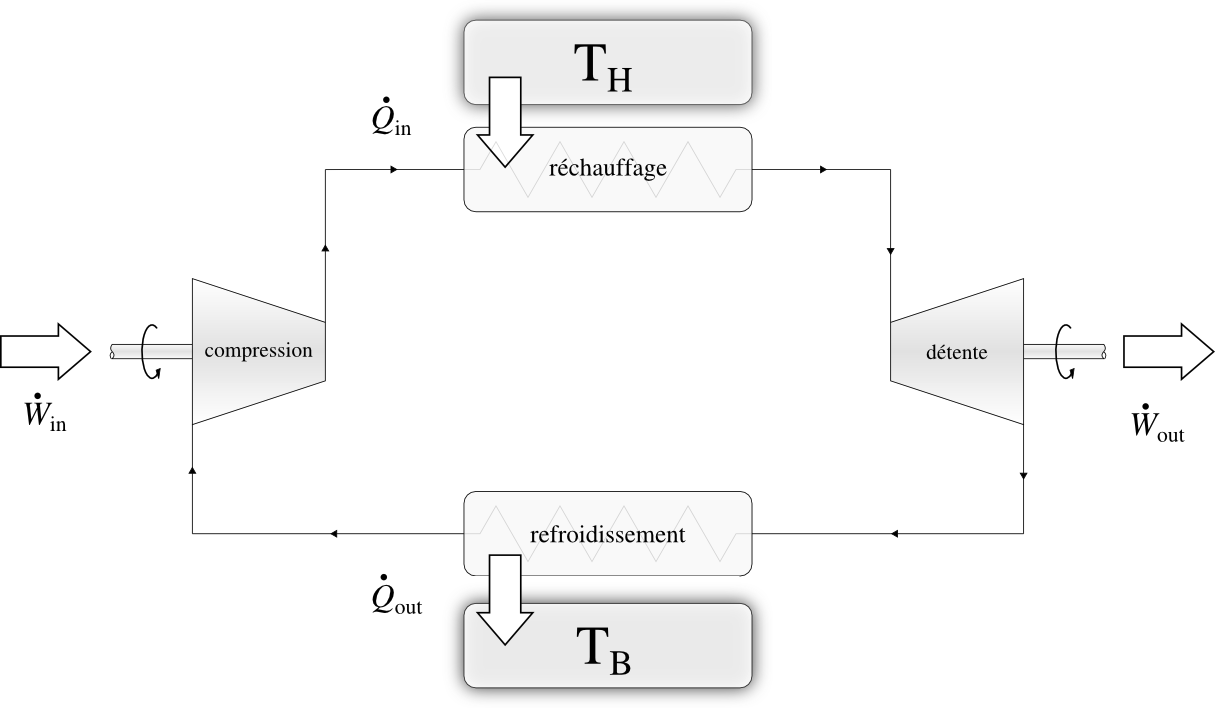
\includegraphics[width=\textwidth]{images/moteur_so.png}
			\end{center}
			\supercaption{Cycle thermodynamique moteur.
				Le fluide absorbe de la chaleur fournie à haute température $T_H$. la puissance de compression est plus faible que la puissance à la détente : la puissance nette sous forme de travail $\dot W_\net = \dot W_\inn + \dot W_\out$ est négative.}{schéma \cczero \oc}
			\label{fig_cycle_thermodynamique_du_moteur_so}
		\end{figure}

		\begin{figure}
			\begin{center}
				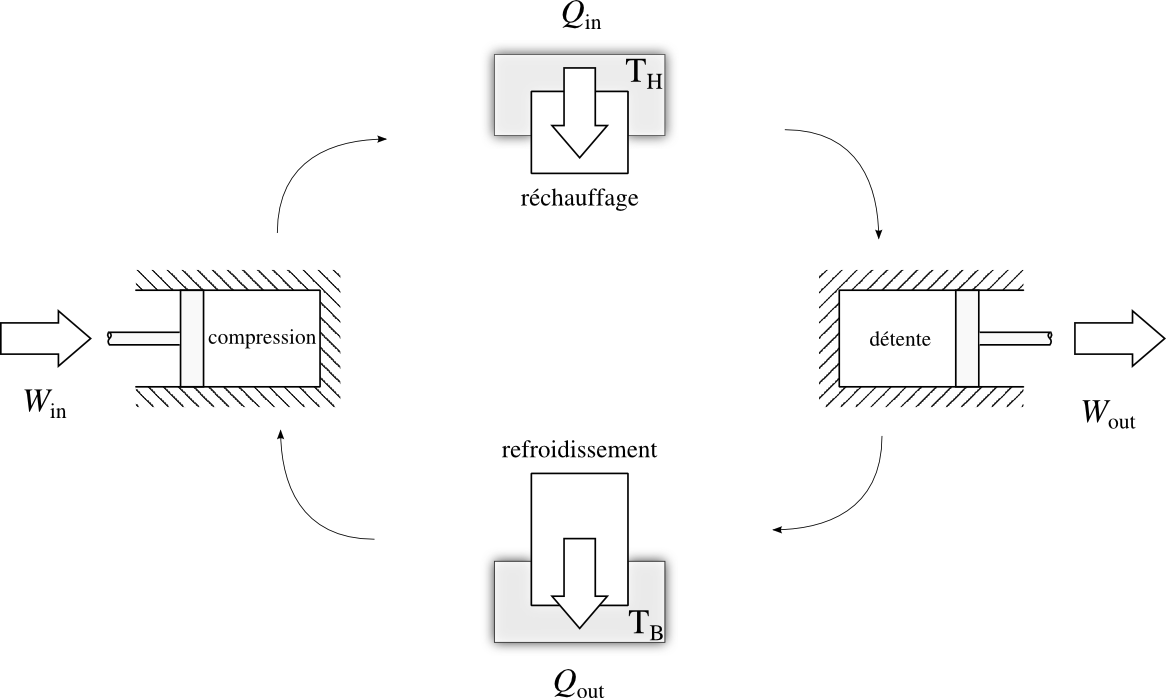
\includegraphics[width=\textwidth]{images/moteur_sf.png}
			\end{center}
			\supercaption{Cycle thermodynamique moteur effectué en séparant les étapes dans le temps (plutôt que dans l’espace comme représenté en \cref{fig_cycle_thermodynamique_du_moteur_so}). Le fluide est réchauffé par une source de chaleur à haute température $T_H$. Le travail net $W_\net = W_\inn + W_\out$ est négatif.}{schéma \cczero \oc}
			\label{fig_cycle_thermodynamique_du_moteur_sf}
		\end{figure}

		Il est possible de lier mécaniquement les sections consommant et fournissant de l’énergie sous forme de travail. Dans le cas où le fluide circule en continu, on peut lier le compresseur et la turbine par un même axe, comme représenté en \cref{fig_cycle_thermodynamique_du_moteur_axe_so}. Dans le cas où les évolutions sont séparées dans le temps, comme dans un moteur à explosion, on peut lier les évolutions en effectuant plusieurs cycles déphasés simultanément (avec plusieurs cylindres) ou en stockant de l’énergie dans un volant d’inertie. Le moteur ne reçoit alors pas de travail extérieur et on obtient alors à sa sortie une puissance $\dot W_\net$.

		\begin{figure}
			\begin{center}
				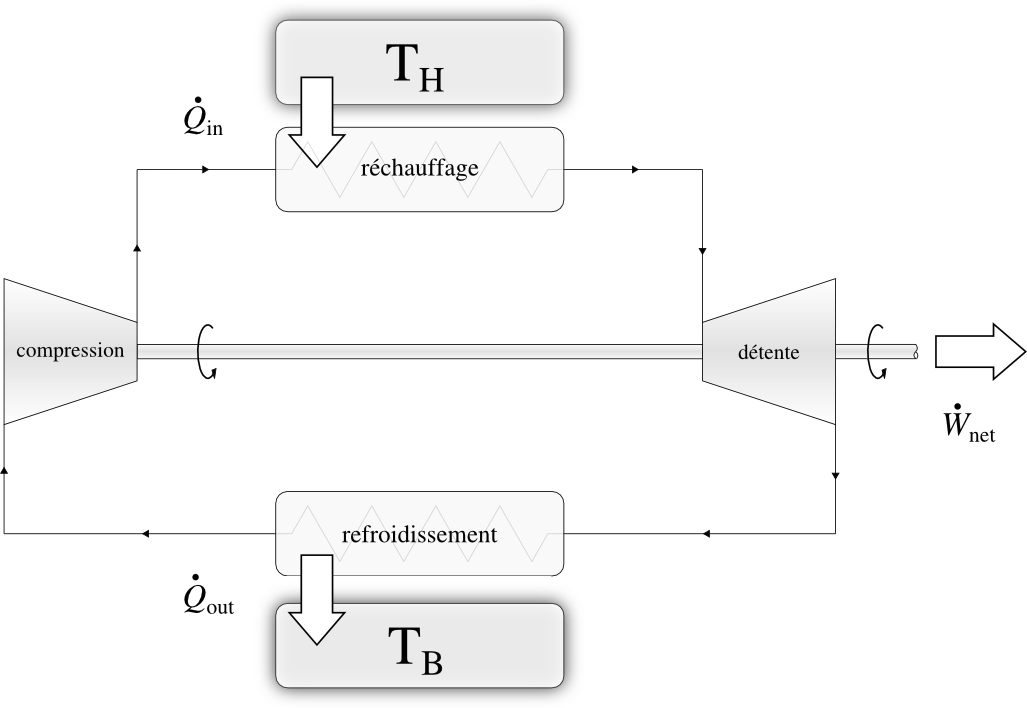
\includegraphics[width=\textwidth]{images/moteur_so_travail_net.png}
			\end{center}
			\supercaption{Cycle thermodynamique moteur, pour lequel le compresseur et la turbine sont reliés mécaniquement. Comme la turbine fournit une puissance $\dot W_\out$ supérieure à celle consommée par le compresseur ($\dot W_\inn$), elle est capable non seulement de l’entraîner mais aussi de fournir un excédent $\dot W_\net$ vers l’extérieur.}{schéma \cczero \oc}
			\label{fig_cycle_thermodynamique_du_moteur_axe_so}
		\end{figure}


	\subsection{Extraire de la chaleur avec du travail}
	\label{ch_principe_fonctionnement_réfrigérateur}

			Lorsque l’on fournit du travail à un fluide, sa température augmente\footnote{Ce n’est pas strictement vrai pour les liquides/vapeurs qui, comme nous l’avons vu dans le \courscinq, connaissent une phase à température constante entre leurs points de saturation – toutefois, ils suivent cette tendance.} et il peut ainsi fournir de la chaleur à un corps qui était initialement à plus haute température («~plus chaud~») que lui.

			À l’inverse, lorsque l’on détend un fluide, sa température baisse et il peut ainsi capter de la chaleur à un corps qui était initialement «~plus froid~» que lui.

			En effectuant ces étapes l’une après l’autre, nous obtenons un \vocab{cycle de réfrigération} : une machine capable de prélever de la chaleur à basse température et de la rejeter à haute température. Un tel cycle est représenté en \cref{fig_refrigerateur_climatiseur_thermopompe_so} (étapes séparées dans l’espace) et \ref{fig_refrigerateur_climatiseur_thermopompe_sf} (étapes séparées dans le temps).
			
			Un examen attentif de ces deux figures réserve une surprise de taille : il s’agit exactement du même agencement que pour un moteur ! La seule différence porte sur les températures de fonctionnement. La température atteinte pendant la compression doit être \textbf{supérieure à la température haute $T_H$}, et la température atteinte pendant la détente doit être \textbf{inférieure à la température basse $T_B$}. Si ces conditions ne sont pas respectées, alors les transferts de chaleur ne peuvent pas se faire dans le sens voulu.
			
			\begin{figure}
				\begin{center}
					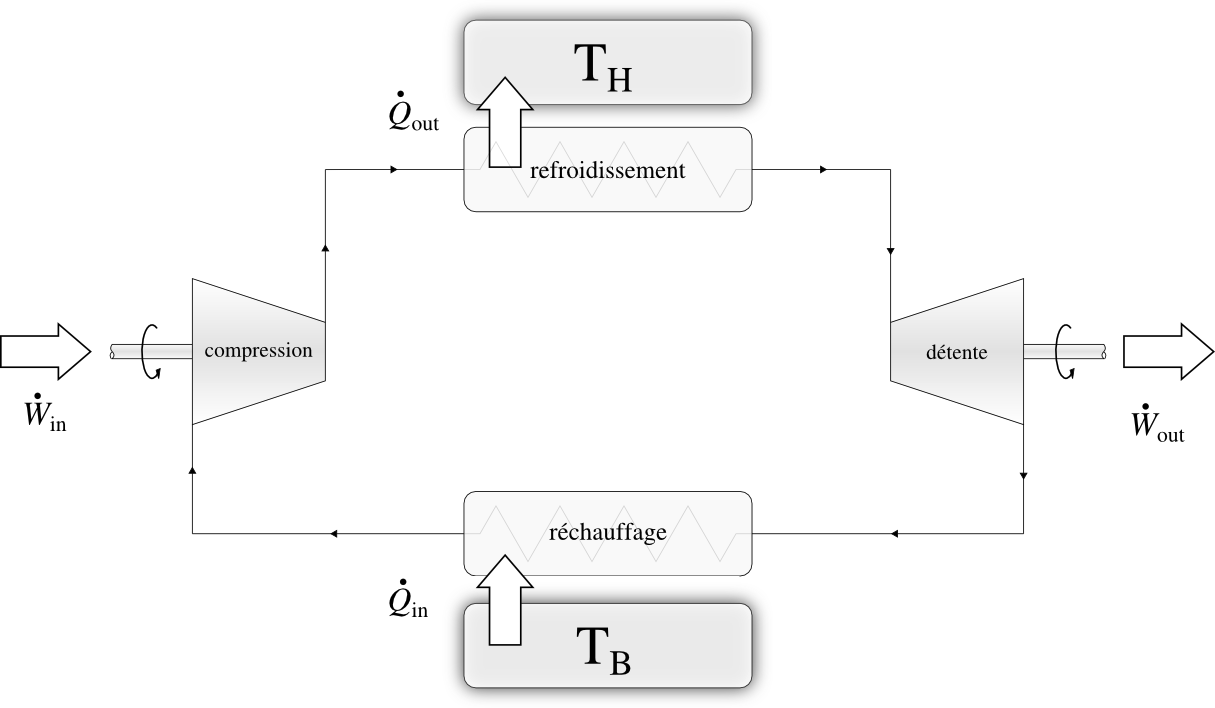
\includegraphics[width=\textwidth]{images/refrigerateur_climatiseur_thermopompe_so.png}
				\end{center}
				\supercaption{Cycle thermodynamique de refroidissement, utilisé dans les réfrigérateurs, climatiseurs et pompes à chaleur.\\
					Une puissance $\dot Q_\inn$ sous forme de chaleur est captée à basse température (le fluide est réchauffé) tandis qu’une puissance $\dot Q_\out$ est rejetée à haute température (le fluide est alors refroidi).}{schéma \cczero \oc}
				\label{fig_refrigerateur_climatiseur_thermopompe_so}
			\end{figure}

			\begin{figure}
				\begin{center}
					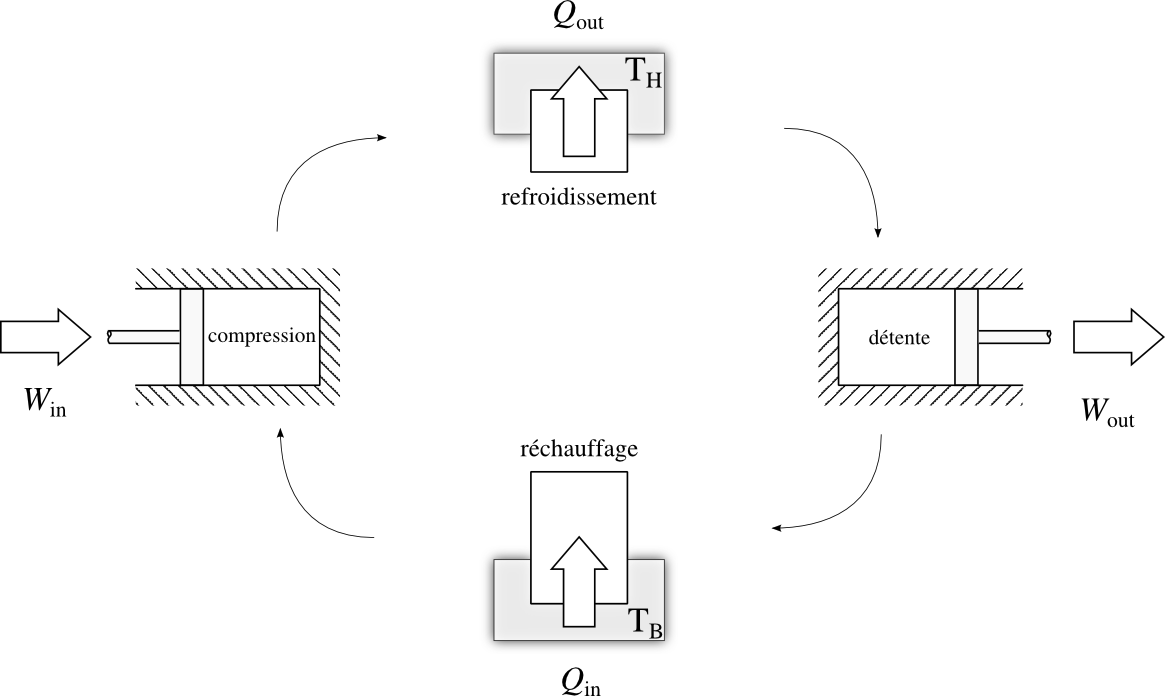
\includegraphics[width=\textwidth]{images/refrigerateur_climatiseur_thermopompe_sf.png}
				\end{center}
				\supercaption{Cycle de réfrigération effectué en séparant les étapes dans le temps (plutôt que dans l’espace comme représenté en \cref{fig_refrigerateur_climatiseur_thermopompe_so})}{schéma \cczero \oc}
				\label{fig_refrigerateur_climatiseur_thermopompe_sf}
			\end{figure}

			Dans un cycle de réfrigération, le fluide a un plus grand volume lorsqu’il est compressé (après avoir été réchauffé) que lorsqu’il est détendu (après avoir été refroidi) : ainsi la compression demande plus de puissance que la détente. La puissance nette $\dot W_\net$ sous forme de travail est donc positive, c’est-à-dire que la machine doit être alimentée en travail par l’extérieur.

			En pratique dans les systèmes de réfrigération, on a souvent recours à une astuce pour faire chuter la température : au lieu d’une turbine, on utilise une simple soupape (parfois appelée \vocab{détendeur}). Cet élément sans pièce mobile ne permet pas de dégager de travail (il augmente donc la puissance consommée par la machine), mais il est beaucoup plus simple de fabrication et d’utilisation.

			La soupape, en termes thermodynamiques, permet d’effectuer une détente entièrement irréversible, augmentant le volume et baissant la pression sans extraire de travail. Si l’on utilisait un gaz parfait, cela n’aurait aucun effet sur la température\footnote{Revoir à ce propos les expériences de Joule et Gay-Lussac étudiées en \S\ref{ch_principe_de_joule}.} et donc aucun intérêt ; mais lorsque l’on utilise des liquides/vapeurs, la détente en soupape est un moyen technologiquement simple de faire chuter la température. Cette modification est décrite en \cref{fig_principe_du_réfrigérateur_soupape}.

			\begin{figure}
				\begin{center}
					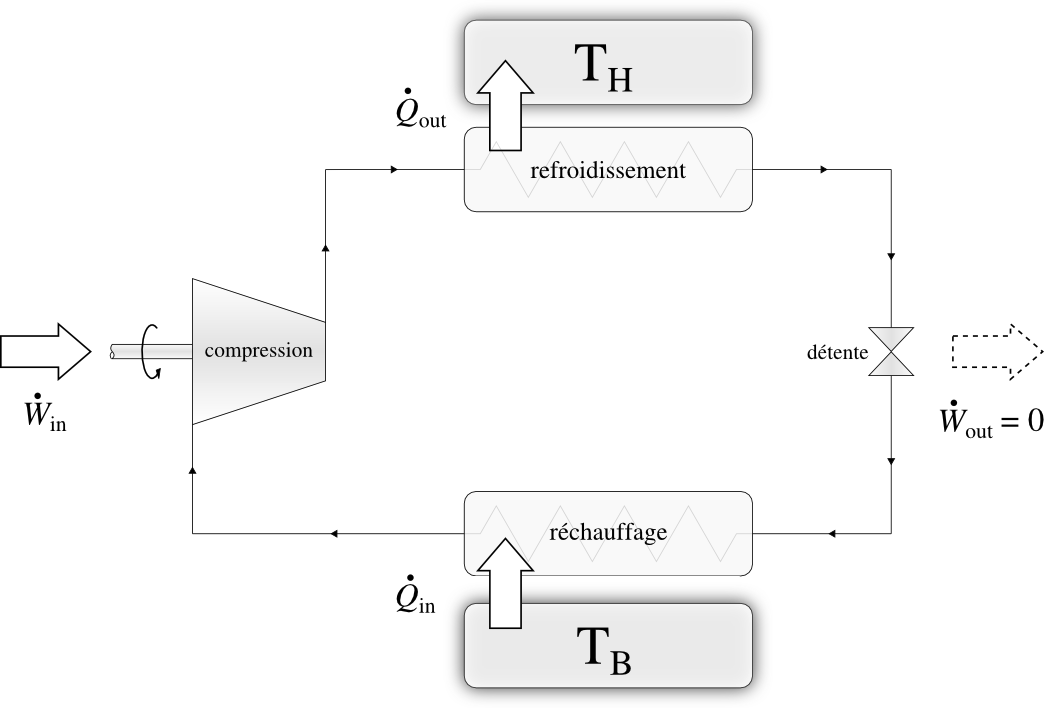
\includegraphics[width=\textwidth]{images/refrigerateur_climatiseur_thermopompe_so_soupape.png}
				\end{center}
				\supercaption{Cycle de réfrigération modifié.
					Lorsque l’on utilise des liquides/vapeurs, il est possible de se dispenser d’extraire du travail lors de la détente. L’utilisation d’une simple soupape suffit pour faire baisser la température du fluide.}{schéma \cczero \oc}
				\label{fig_principe_du_réfrigérateur_soupape}
			\end{figure}

			\clearfloats
			Les cycles de réfrigération ont deux grands types d’application :
			\begin{description}
				\item[Les pompes à chaleur] appelées aussi \vocab{thermopompes} (\cref{fig_agencement_thermopompe}) sont agencées de façon à rejeter la chaleur vers un corps à haute température, le plus souvent une habitation ;
				\item[Les réfrigérateurs et climatiseurs] (\cref{fig_agencement_refrigerateur_climatiseur}) sont agencés de façon à extraire de la chaleur d’un corps à basse température, le plus souvent une chambre froide.
			\end{description}

			Dans ces deux types d’application, il s’agit exactement de la même machine, fonctionnant avec le même cycle. La seule différence concerne l’agencement intérieur/extérieur des composants : une pompe à chaleur n’est ni plus ni moins qu’un réfrigérateur positionné de sorte qu’il «~refroidisse l’extérieur~».

			\begin{figure}
				\begin{center}
					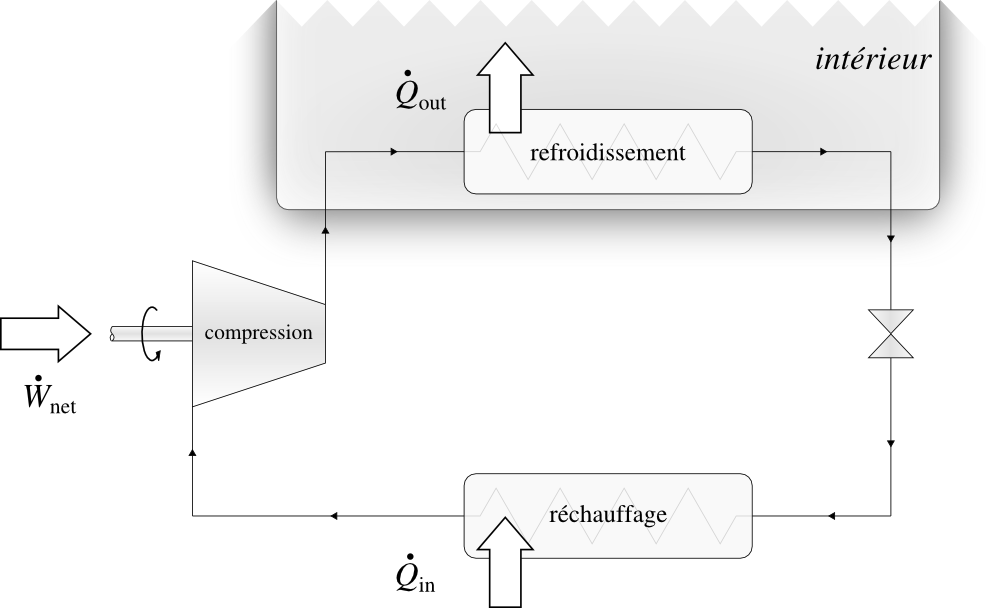
\includegraphics[width=\textwidth]{images/agencement_thermopompe.png}
				\end{center}
				\supercaption{Agencement d’une pompe à chaleur. La machine est positionnée de sorte à refouler à l’intérieur (où la température est plus haute) la chaleur prélevée à l’extérieur (où la température est plus basse).}{schéma \cczero \oc}
				\label{fig_agencement_thermopompe}
			\end{figure}
			
			\begin{figure}
				\begin{center}
					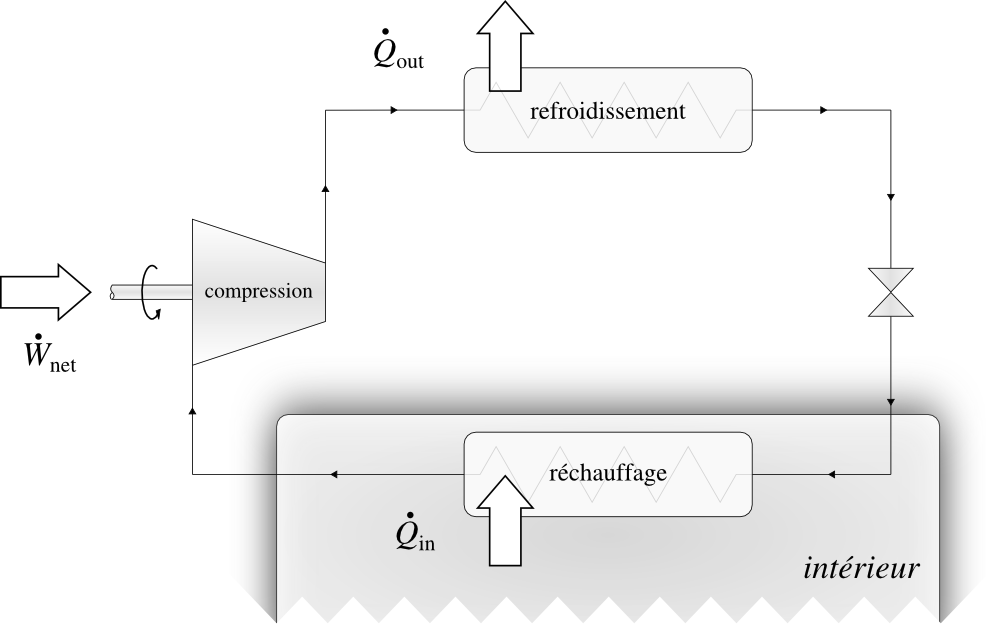
\includegraphics[width=\textwidth]{images/agencement_refrigerateur_climatiseur.png}
				\end{center}
				\supercaption{Agencement d’un réfrigérateur ou d’un climatiseur. La machine est positionnée de sorte à refouler à l’extérieur (où la température est plus haute) la chaleur prélevée à l’intérieur (où la température est plus basse). Il s’agit exactement de la même machine qu’en \cref{fig_agencement_thermopompe}.}{schéma \cczero \oc}
				\label{fig_agencement_refrigerateur_climatiseur}
			\end{figure}

			\clearfloats
			La similarité entre climatiseur et pompe à chaleur permet d’effectuer ces deux fonctions avec une seule même machine, que l’on dit alors \vocab{inversable} – ou parfois \vocab{réversible}, à tort comme nous le verrons au \courssept. En fonction des besoins, le sens de circulation du fluide est inversé, ce qui provoque l’inversion des transferts de chaleur. Ce type de machine est représenté en \cref{fig_agencement_thermopompe_climatiseur_inversable}.
			
			\begin{figure}
				\begin{center}
					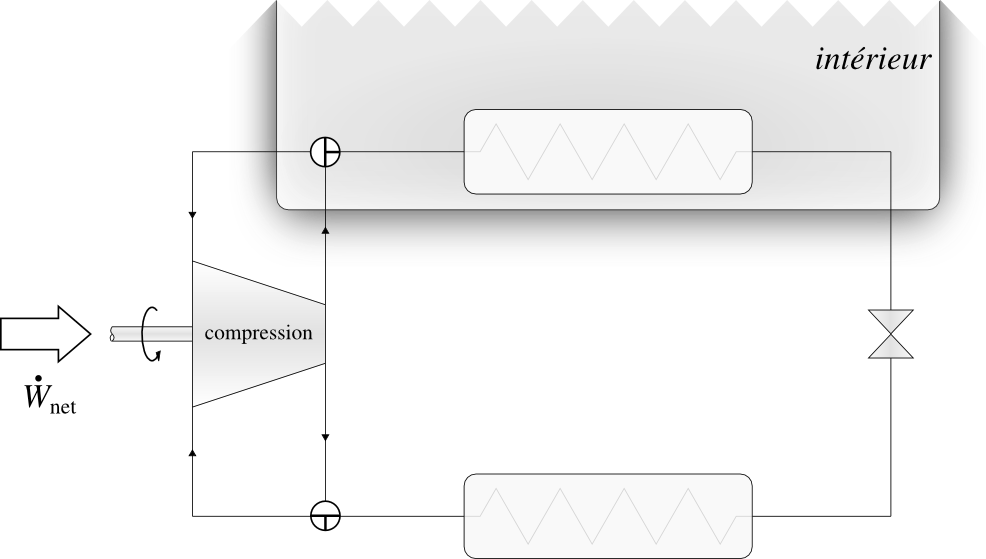
\includegraphics[width=\textwidth]{images/agencement_thermopompe_climatiseur_inversable.png}
				\end{center}
				\supercaption{Agencement d’un climatiseur inversable. En pivotant des deux vannes de~\SI{90}{\degree} dans le sens anti-horaire, on change la fonction depuis une pompe à chaleur vers un climatiseur.}{schéma \cczero \oc}
				\label{fig_agencement_thermopompe_climatiseur_inversable}
			\end{figure}


\section{Rendement des cycles}

	Le \vocab{rendement}\footnote{Dans le présent ouvrage, nous utilisons indistinctement les termes \textit{efficacité} et \textit{rendement}. Toutefois, certains auteurs font une distinction entre l’efficacité $\eta$ définie en~\ref{def_efficacité_machines_thermiques} et un rendement $R \equiv \frac{\eta_\text{réele}}{\eta_\text{théorique}}$ comparant l’efficacité atteinte en pratique avec l’efficacité maximale atteignable par la machine. Il faut alors soigneusement défnir les hypothèses associées au calcul de l’efficacité maximale.}%
	 ou l’\vocab{efficacité} $\eta$ d’une machine thermique compare le transfert ou la transformation utile qu’elle effectue avec le coût énergétique qu’elle engendre. Nous retiendrons la définition de principe suivante :
	\begin{equation}
		\eta \equiv \left| \frac{\text{transfert utile}}{\text{dépense énergétique}} \right|
		\label{def_efficacité_machines_thermiques}
	\end{equation}

	Par convention le rendement est toujours exprimé sous la forme d’un nombre positif ; ainsi nous utilisons une valeur absolue dans l’\cref{def_efficacité_machines_thermiques}. Pour chacun des trois types de machines thermiques, nous allons définir et quantifier ce «~transfert utile~» et cette «~dépense énergétique~».


	\subsection{Rendement d’un moteur}
	\label{ch_rendement_moteur}

		La fonction d’un moteur thermique, comme ceux que l’on trouve à bord des automobiles ou dans les centrales électriques, est de produire du travail, c’est-à-dire une quantité $\dot W_\net$ négative (\cref{fig_transferts_moteur}). La dépense engendrée pour générer ce travail est la chaleur qu’il reçoit, c’est-à-dire la quantité $\dot Q_\inn$ (provenant usuellement de la combustion de carburant ou de la fission de noyaux atomiques).

		\begin{figure}
			\begin{center}
				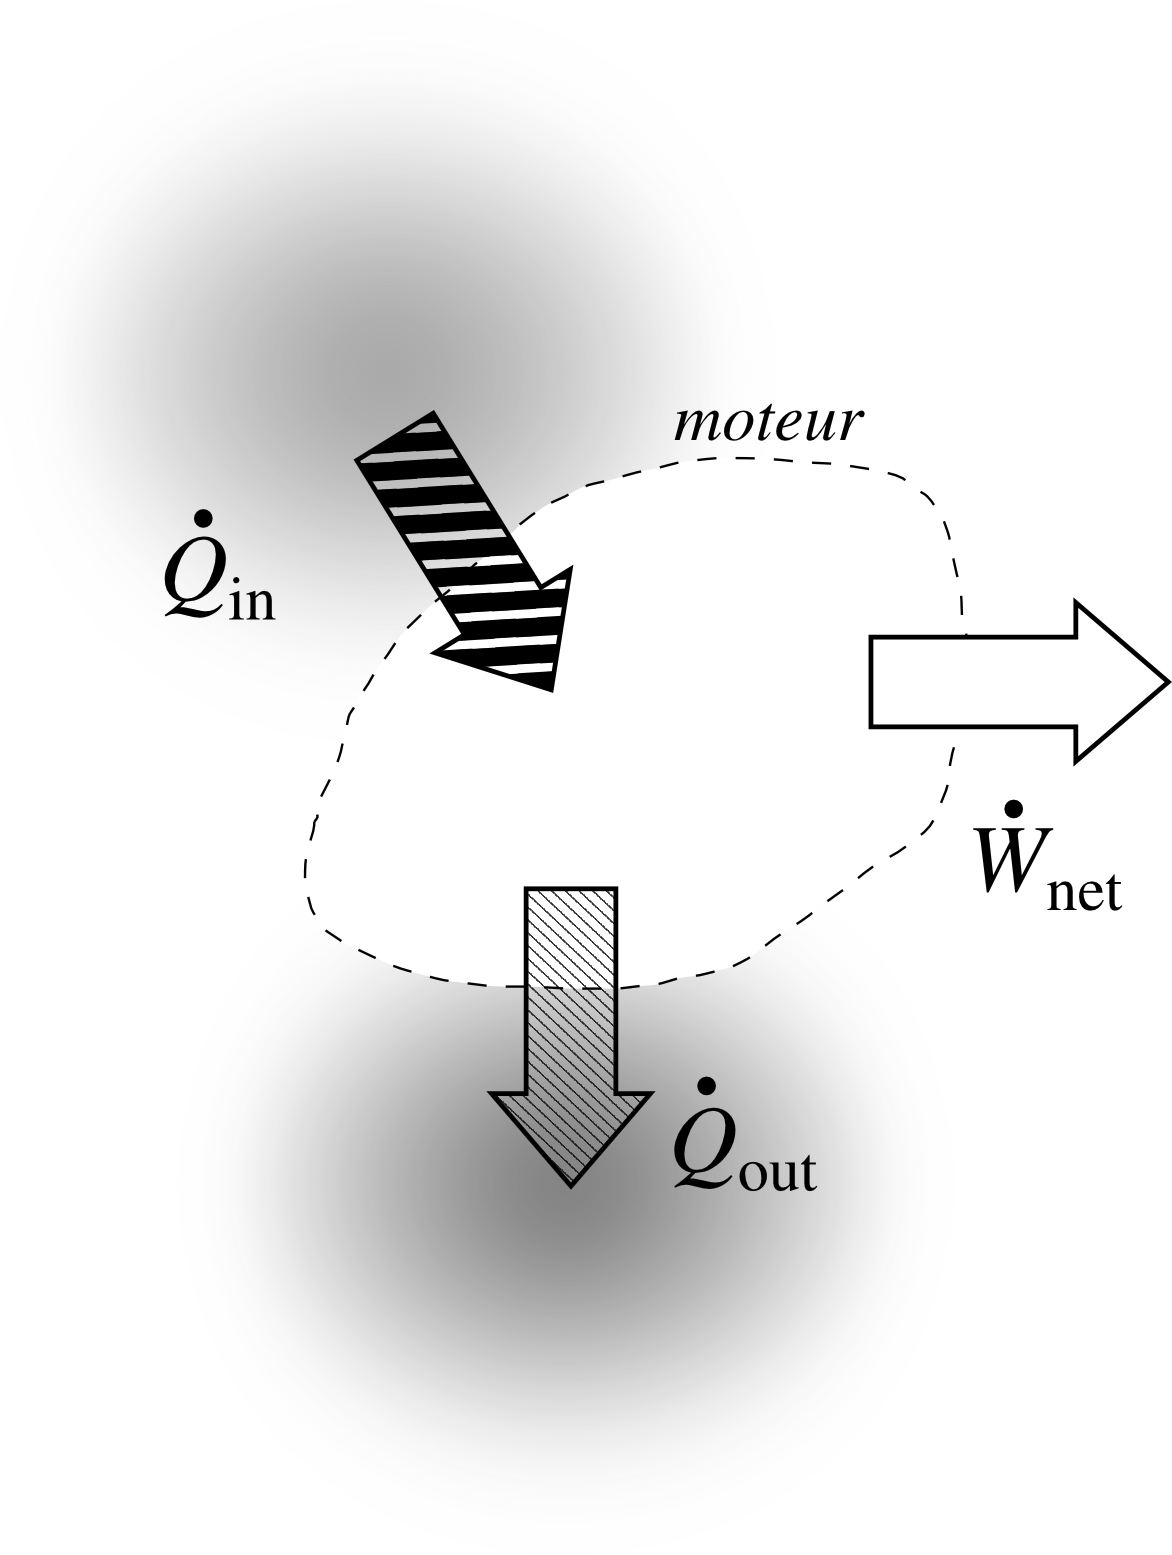
\includegraphics[height=10cm]{images/efficacite_moteur.png}
			\end{center}
			\supercaption{Transferts énergétiques associés à un moteur.
				On souhaite obtenir un grand transfert $\dot W_\net$  (résultat) à partir du transfert $\dot Q_\inn$ (coût).
				Le rejet $\dot Q_\out$ est indésirable.}{schéma \cczero \oc}
			\label{fig_transferts_moteur}
		\end{figure}

		D’après la définition~\ref{def_efficacité_machines_thermiques} le rendement $\eta_\text{moteur}$ du moteur thermique est donc :
		\begin{equation}
			\eta_\text{moteur} \equiv \left| \frac{\dot W_\net}{\dot Q_\inn} \right|
			\label{def_rendement_moteur}
		\end{equation}

		\begin{anexample}
			Un moteur automobile reçoit une puissance de~\SI{100}{\kilo\watt} sous forme de chaleur issue de la combustion d’essence ; il fournit \SI{55}{\kilo\watt} sous forme de travail à l’arbre de transmission. Quel est son rendement ?
	
			\begin{answer}
				Le rendement est de $\eta_\text{moteur} = \left| \frac{\dot W_\net}{\dot Q_\inn} \right| = \left| \frac{\num{-55e3}}{\num{+100e3}} \right| = \num{0,55} = \SI{55}{\percent}$.
					\begin{remark} Ce moteur effectue un rejet $\dot Q_\out = -\dot W_\net - \dot Q_\inn = -(\num{-55e3}) - \num{100e3}= \SI{-45}{\kilo\watt}$. Cette chaleur est en majeure partie évacuée par le pot d’échappement.\end{remark}
					\begin{remark} On se doute bien qu’il faudra toujours fournir au moins autant de chaleur $\dot Q_\inn$ que le moteur ne fournit de travail $\dot W_\net$ ; le rendement d’un moteur sera donc toujours nécessairement inférieur à~\num{1}.\end{remark}
			\end{answer}
		\end{anexample}

		La puissance nette $\dot W_\net$ sous forme de travail peut être exprimée en fonction des autres transferts énergétiques, et ainsi :
		\begin{IEEEeqnarray}{rCl}
			\dot W_\net 			& = & \dot W_\inn + \dot W_\out = -\dot Q_\inn - \dot Q_\out	\nonumber \\
			\eta_\text{moteur} 	& = & 1 - \left| \frac{\dot Q_\out}{\dot Q_\inn} \right|	\label{eq_rendement_moteur_qin_qout}
		\end{IEEEeqnarray}

		Cette \cref{eq_rendement_moteur_qin_qout} nous sera fort utile au chapitre prochain (\S\ref{ch_efficacité_moteur_carnot}), où nous voudrons lier les transferts de chaleur $\dot Q_\inn$ et $\dot Q_\out$ aux températures auxquelles ils sont effectués.



	\subsection{Rendement d’un réfrigérateur ou d’un climatiseur}
	\label{ch_rendement_réfrigérateur}

		La fonction d’un réfrigérateur ou d’un climatiseur est d’extraire de la chaleur, c’est-à-dire de générer une puissance $\dot Q_\inn$ (chaleur extraite chaque seconde du compartiment à refroidir) de signe positif. Ce transfert (\cref{fig_transferts_réfrigérateur}) est rendu possible par l’apport au réfrigérateur d’un travail, $\dot W_\net$ , une «~dépense~» nécessairement positive.

		\begin{figure}
			\begin{center}
				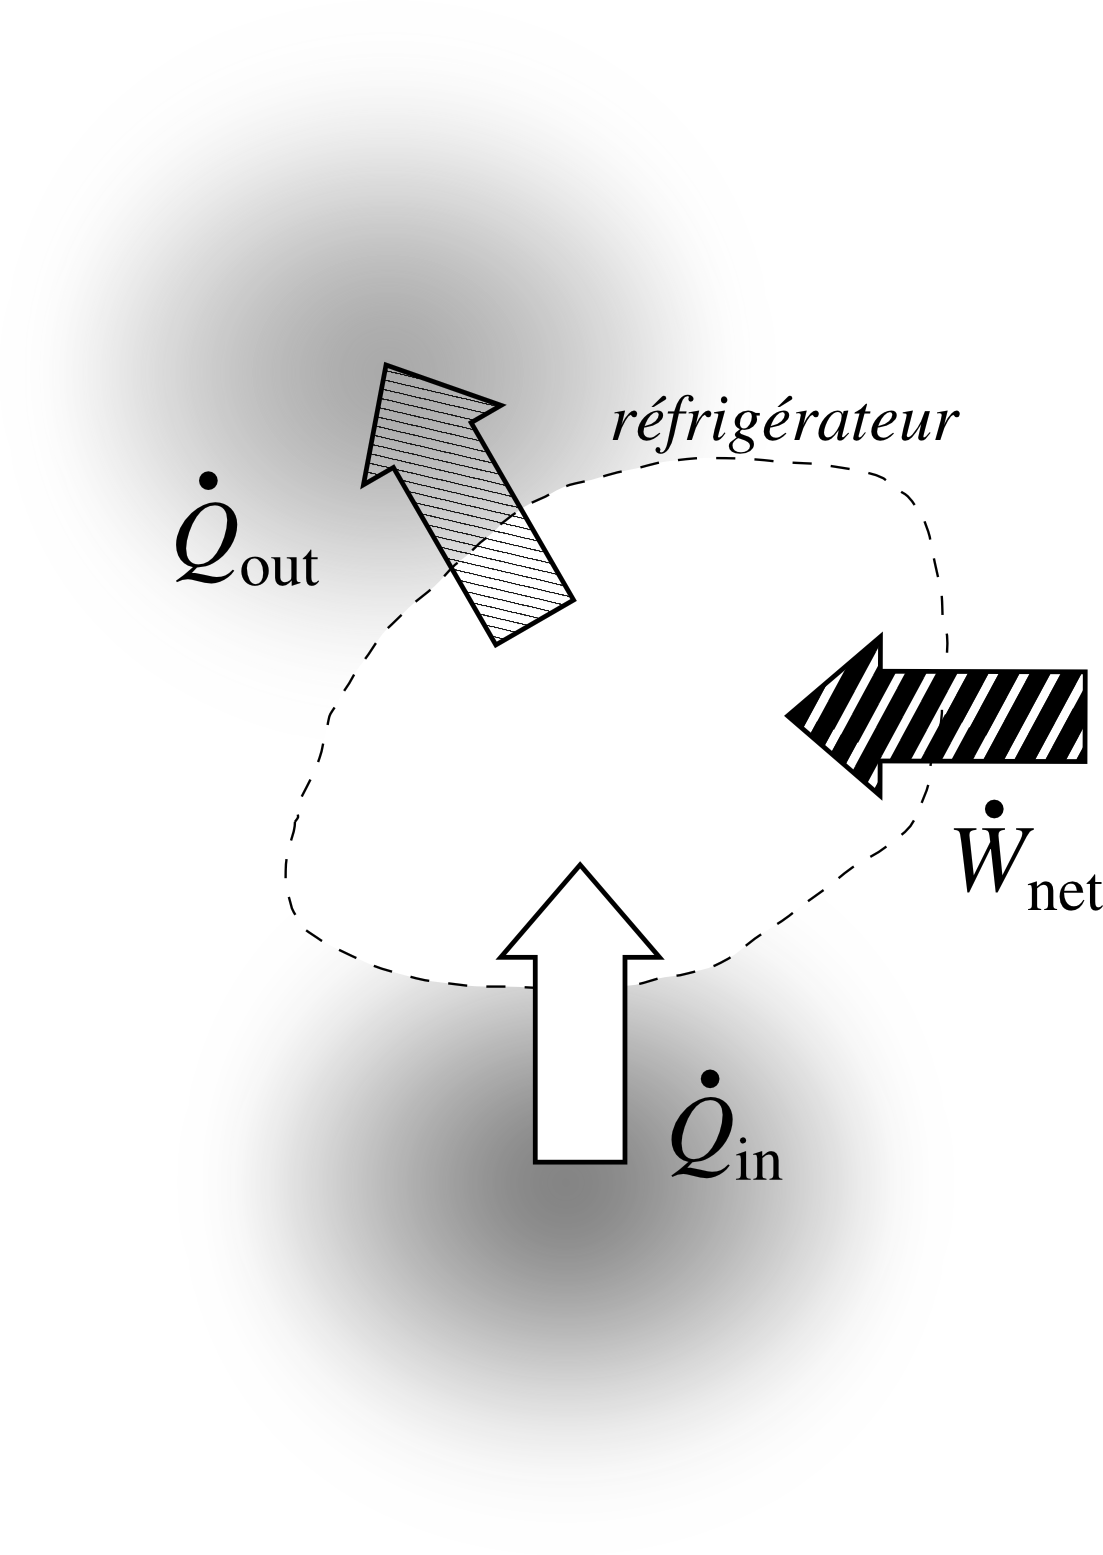
\includegraphics[height=10cm]{images/efficacite_refrigerateur_climatiseur.png}
			\end{center}
			\supercaption{Transferts énergétiques associés à un réfrigérateur ou à un climatiseur.
				On souhaite obtenir un grand transfert $\dot Q_\inn$ (résultat) à partir du transfert $\dot W_\net$ (coût).}{schéma \cczero \oc}
			\label{fig_transferts_réfrigérateur}
		\end{figure}

		D’après la définition~\ref{def_efficacité_machines_thermiques} le rendement (dit aussi parfois \vocab{coefficient of performance}, ou $\textsc{cop}_\text{réfrigération}$) d’un réfrigérateur ou d’un climatiseur est donc :
		\begin{equation}
			\eta_\text{réfrigérateur} = \eta _\text{climatiseur} \equiv \left| \frac{\dot Q_\inn}{\dot W_\net} \right|
			\label{def_rendement_climatiseur_refrigerateur}
		\end{equation}

		\begin{anexample}
			Un réfrigérateur consomme une puissance électrique de~\SI{100}{\watt} ; il extrait de la chaleur de la chambre froide avec une puissance de~\SI{120}{\watt}. Quel est son rendement ?
	
			\begin{answer}
				Le rendement est de $\eta_\text{réfrigérateur} = \left| \frac{\dot Q_\inn}{\dot W_\net} \right| = \left| \frac{\num{+120}}{\num{+100}} \right| = \num{1,2} = \SI{120}{\percent}$.
					\begin{remark} Ce réfrigérateur effectue un rejet $\dot Q_\out = -\dot W_\net - \dot Q_\inn = \num{-100} - \num{120}= \SI{-220}{\watt}$ à l’extérieur de la chambre froide (usuellement, dans l’habitation elle-même).\end{remark}
					\begin{remark} Les réfrigérateurs et climatiseurs domestiques ont souvent un rendement supérieur à~\num{1} mais en fonction des températures demandées, le rendement peut tout à fait y être inférieur.\end{remark}
			\end{answer}
		\end{anexample}

		En prenant garde aux pièges algébriques associés à l’utilisation de valeurs absolues, pour préparer le chapitre prochain nous pouvons exprimer ce rendement en fonction des transferts de chaleur uniquement :
		\begin{equation}
			\eta _\text{réfrigérateur} = \eta _\text{climatiseur} = \frac{1}{\left| \frac{\dot Q_\out}{\dot Q_\inn} \right| - 1}
			\label{rendement_réfrigérateur_qin_qout}
		\end{equation}





	\subsection{Rendement d’une pompe à chaleur}
	\label{ch_rendement_thermopompe}

		Une pompe à chaleur fonctionne exactement de la même manière qu’un climatiseur. Sa fonction est de générer un transfert $\dot Q_\out$ vers la section «~chaude~» (usuellement l’intérieur d’une habitation). Ce transfert, représenté en \cref{fig_transferts_thermopompe}, est rendu possible par l’apport à la thermopompe de $\dot W_\net$ , une «~dépense~» nécessairement positive.

		\begin{figure}
			\begin{center}
				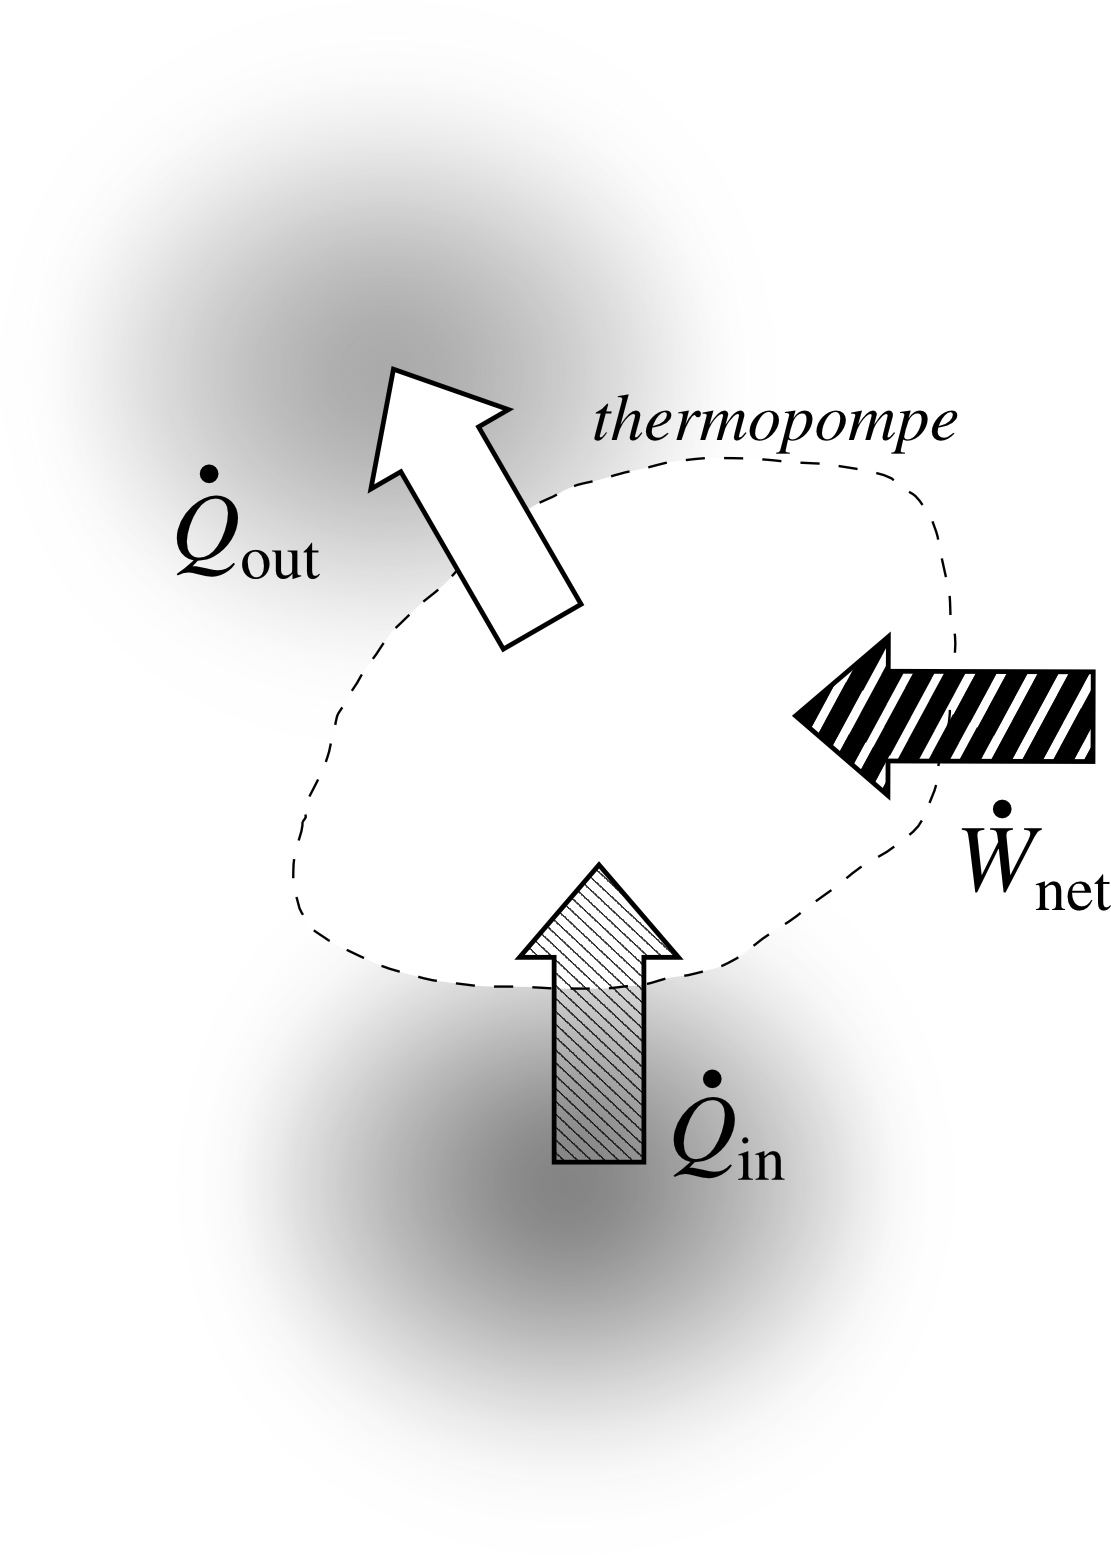
\includegraphics[height=10cm]{images/efficacite_thermopompe.png}
			\end{center}
			\supercaption{Transferts énergétiques associés à une pompe à chaleur.
					On souhaite obtenir un grand transfert $\dot Q_\out$ (résultat) à partir du transfert $\dot W_\net$ (coût).}{schéma \cczero \oc}
			\label{fig_transferts_thermopompe}
		\end{figure}

		Le rendement $\eta_\text{thermopompe}$ (dit aussi $\textsc{cop}_\text{thermopompe}$) de la thermopompe est donc défini par :
		\begin{equation}
			\eta_\text{thermopompe} \equiv \left| \frac{\dot Q_\out}{\dot W_\net} \right|
			\label{def_rendement_thermopompe}
		\end{equation}
	
			\begin{anexample}
				Une pompe à chaleur consomme une puissance électrique de~\SI{100}{\watt} ; elle chauffe l’intérieur d’une pièce avec une puissance de~\SI{350}{\watt}. Quel est son rendement ?
		
				\begin{answer}
					Le rendement est de $\eta_\text{thermopompe} = \left| \frac{\dot Q_\out}{\dot W_\net} \right| = \left| \frac{\num{-350}}{\num{+100}} \right| = \num{3.5}$.
						\begin{remark} La pompe à chaleur rejette plus de chaleur qu’elle ne consomme de travail –\ c’est tout son intérêt. Si le \textsc{cop} était égal ou inférieur à~\num{1}, il serait plus économique et bien plus simple d’utiliser un radiateur électrique.\end{remark}
				\end{answer}
			\end{anexample}


		De la même façon que pour les sections précédentes, on peut exprimer ce rendement en fonction des débits de chaleur uniquement :
		\begin{equation}
			\eta_\text{thermopompe} = \frac{1}{1 - \left| \frac{\dot Q_\inn}{\dot Q_\out} \right|}
			\label{eq_rendement_thermopompe_qin_qout}
		\end{equation}




	\subsection{De la faible performance des machines}

		\thermoquotebegin{O}
			L’on a souvent agité la question de savoir si la puissance motrice de la chaleur est limitée, ou si elle est sans bornes ; si les perfectionnements possibles des machines à feu ont un terme assignable, terme que la nature des choses empêche de dépasser par quelque moyen que ce soit, ou si au contraire ces perfectionnemens sont susceptibles d’une extension indéfinie.
		\thermoquoteend{Sadi Carnot, 1824~\cite{carnot1824}}{}

		Dans tous les cas que nous avons étudiés plus haut, pour chaque cycle, nous avons inclus un transfert indésirable. Dans le cycle moteur, une partie de l’énergie est gâchée sous forme de rejet de chaleur ($\dot Q_\out$). Dans les cycles de réfrigération, on doit apporter du travail ($\dot W_\inn$) pour effectuer un transfert de chaleur qui \textit{a priori} aurait pu sembler «~gratuit~» ($\dot Q_\out$ étant alors égal à $\dot Q_\inn$).

		L’étudiant/e en ingénierie s’indignera certainement de la place qu’occupent ces pertes dans ce chapitre --\ et des timides rendements atteints par les machines décrites en exemple. Pourquoi les rendements calculés dans les exemples et dans les exercices qui suivent sont-ils si faibles, et surtout, comment concevoir des cycles de plus grande efficacité ? Nous aurons soin et à cœur de répondre à ces questions au \courssept.

\atstartofhistorysection
\section[Un peu d’histoire : le nombre de temps moteur]{Un peu d’histoire :\onlyamphibook{\\} le nombre de temps moteur}
\label{ch_deux_temps}

	Historiquement, nous avons appris à transformer de la chaleur en travail en manipulant des quantités fixes de fluide emprisonné dans des enclaves. Ces enclaves ont toujours été de géométrie cylindrique, ce qui facilite grandement la fabrication des pistons qui exploitent les variations de volume du fluide pour en extraire du~travail.
	
	Lorsque le fluide est de l’eau, l’apport de chaleur se fait dans une chaudière et la vapeur est \emph{ensuite} transférée dans le ou les cylindres pour y être détendue (\S\ref{ch_cycles_moteurs_vapeur}). À la fin du \textsc{xix}\ieme siècle toutefois, on commence à utiliser de l’air, un fluide à l’intérieur duquel on peut directement créer la chaleur par combustion. Le processus complexe consistant jusqu’alors à effectuer une combustion séparée pour chauffer une chaudière métallique qui elle-même chauffe enfin l’eau du moteur est éliminé avec toutes les pertes de chaleur et de température qu’il engendre. C’est la naissance du moteur \vocab[moteur!à combustion interne]{à combustion interne}\index{combustion!interne, moteur à}, dont le développement sera notamment porté par les ingénieurs allemands \wf{Nikolaus Otto} et \wf{Rudolf Diesel} (\S\ref{ch_moteurs_alternatifs}). On réalise désormais la combustion et la détente au même endroit, directement dans le cylindre.
	
	Cependant, pour effectuer une combustion interne, il faut résoudre un nouveau problème : comme l’oxygène de l’air est utilisé pendant la combustion, celle-ci ne peut être effectuée qu’une seule fois. Après chaque combustion, il est donc indispensable de rejeter hors du cylindre les produits de réaction ($\text{CO}_2$ et $\text{H}_2\text{O}$ essentiellement) et d’y ré-insérer de l’air «~frais~» contenant l’oxygène $\text{O}_2$ nécessaire à la rupture des molécules d’hydrocarbures $\text{C}_x\text{H}_y$ produisant la chaleur. Deux solutions différentes sont alors adoptées.
	
	La méthode la plus courante est de consacrer un mouvement de piston à chaque étape : le premier pour la compression, le second pour la détente (après ou pendant la combustion), le troisième pour rejeter les gaz brûlés (échappement), et le dernier pour admettre de l’air frais (aspiration). Les moteurs suivant ce procédé sont dits \vocab[moteur!à quatre temps]{à quatre temps}\index{temps moteur!quatre temps} (\cref{fig_quatre_temps}), et ils ont toujours été les plus utilisés.
	
	\onlyamphibook{\begin{figure}[htb!]}%handmade
	\onlyframabook{\begin{figure}}
		\begin{center}
			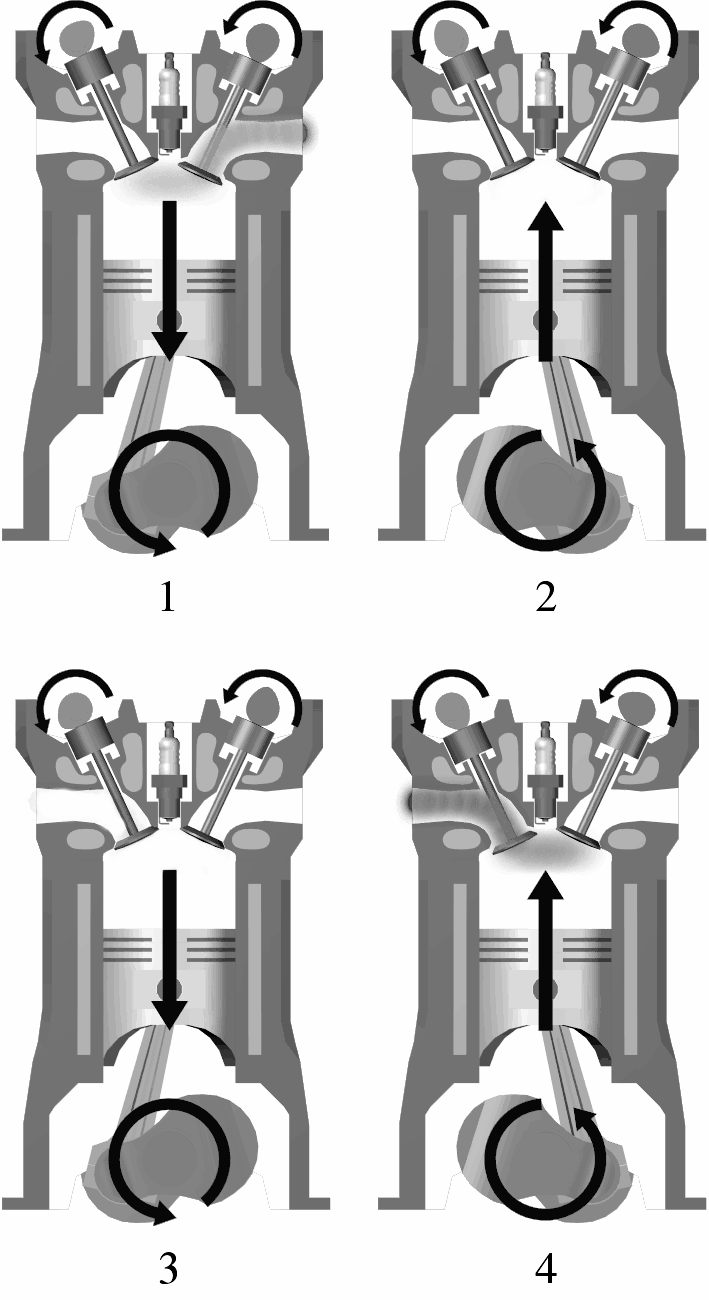
\includegraphics[width=6cm]{images/four_stroke_cycle.png}
			\supercaption{Les quatre étapes d’un moteur à quatre temps. Le piston descend pour admettre de l’air frais arrivant de la droite (\vocab[admission (temps moteur)]{admission}\index{temps moteur!admission}, 1) ; il monte ensuite pour augmenter la température de l’air (\vocab[compression (temps moteur)]{compression}\index{temps moteur!compression}, 2) ; la production de travail utile a lieu pendant une descente (\vocab[détente (temps moteur)]{détente}\index{temps moteur!détente}, 3) ; enfin l’air est rejeté à l’extérieur lors d’un quatrième et dernier mouvement (\vocab[échappement (temps moteur)]{échappement}\index{temps moteur!détente}), 4) avant de recommencer le cycle. La plupart des moteurs à pistons-cylindres actuels suivent ce procédé.}%
			{schémas \wcfile{Four stroke cycle intake.png}{1} \wcfile{Four stroke cycle compression.png}{2} \wcfile{Four stroke cycle power.png}{3} \wcfile{Four stroke cycle exhaust.png}{4} \ccby par \weun{Wapcaplet}{Eric Pierce}}
			\label{fig_quatre_temps}
		\end{center}
	\end{figure}
	
	La seconde méthode ne manquera pas de surprendre les puristes : il s’agit d’effectuer ces quatre opérations en \vocab[moteur!à deux temps]{deux temps}\index{temps moteur!deux temps} seulement. Dans ces moteurs, une partie de l’expansion des gaz est consacrée à leur échappement, qui est effectué simultanément à l’admission d’air (figures~\ref{fig_cycle_deux_temps} et~\ref{fig_pv_deux_temps}). Assurément, aucune des quatre étapes ne peut être effectuée de façon optimale : les phases de compression et détente ne sont effectuées que sur une partie du débattement, et la vidange est nécessairement incomplète à cause du mélange des gaz frais et usagés. Par contre, les combustions sont deux fois plus fréquentes, puisqu’on se dispense des temps d’admission et d’échappement pendant lesquels aucune opération thermodynamique n’a lieu. Ainsi, à cylindrée et vitesse de rotation égales, les moteurs à deux temps sont beaucoup plus puissants que leurs homologues à quatre temps, même s’ils sont aussi nettement moins efficaces.
	
	\begin{figure}
		\begin{center}
			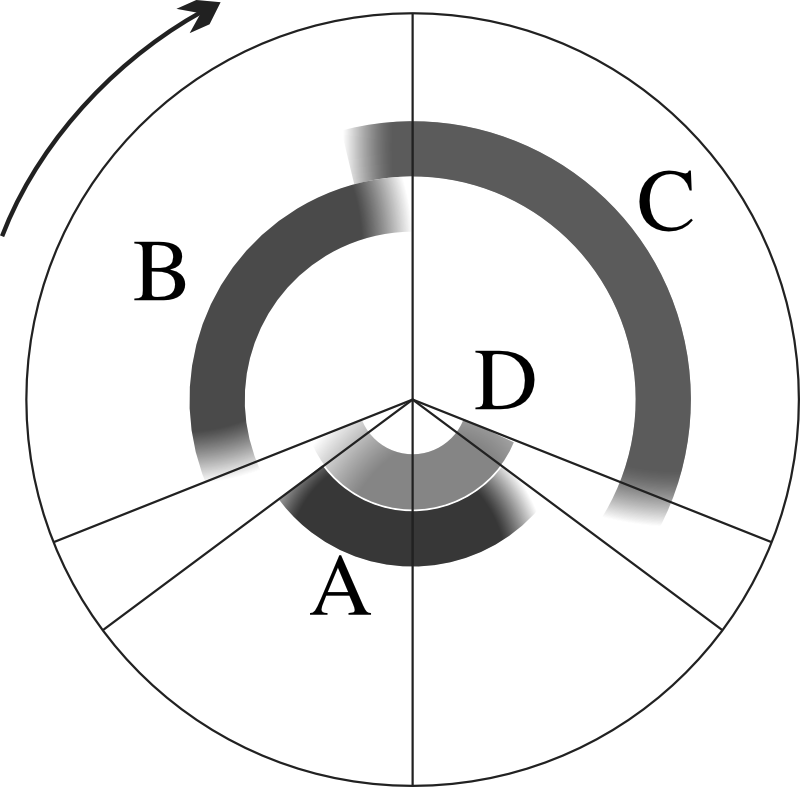
\includegraphics[width=6cm]{images/cycle_deux_temps.png}
			\supercaption{Cycle d’un moteur deux-temps. Les quatre étapes nécessaires au fonctionnement sont effectuées sur une seule révolution de vilebrequin, soit deux mouvements de piston. L’admission (A) se fait pendant le passage au point mort bas, la compression (B) débute tard et la détente (C) est interrompue pour permettre la vidange (D) lorsque le piston se rapproche à nouveau du point mort~bas.}%
			{schéma dérivé d’\wcfile{Ciclo del motore 2T unidirezionale.svg}{un schéma} \ccbysa par \wcu{A7N8X}}
			\label{fig_cycle_deux_temps}
		\end{center}
	\end{figure}	
	
	\begin{figure}
		\begin{center}
			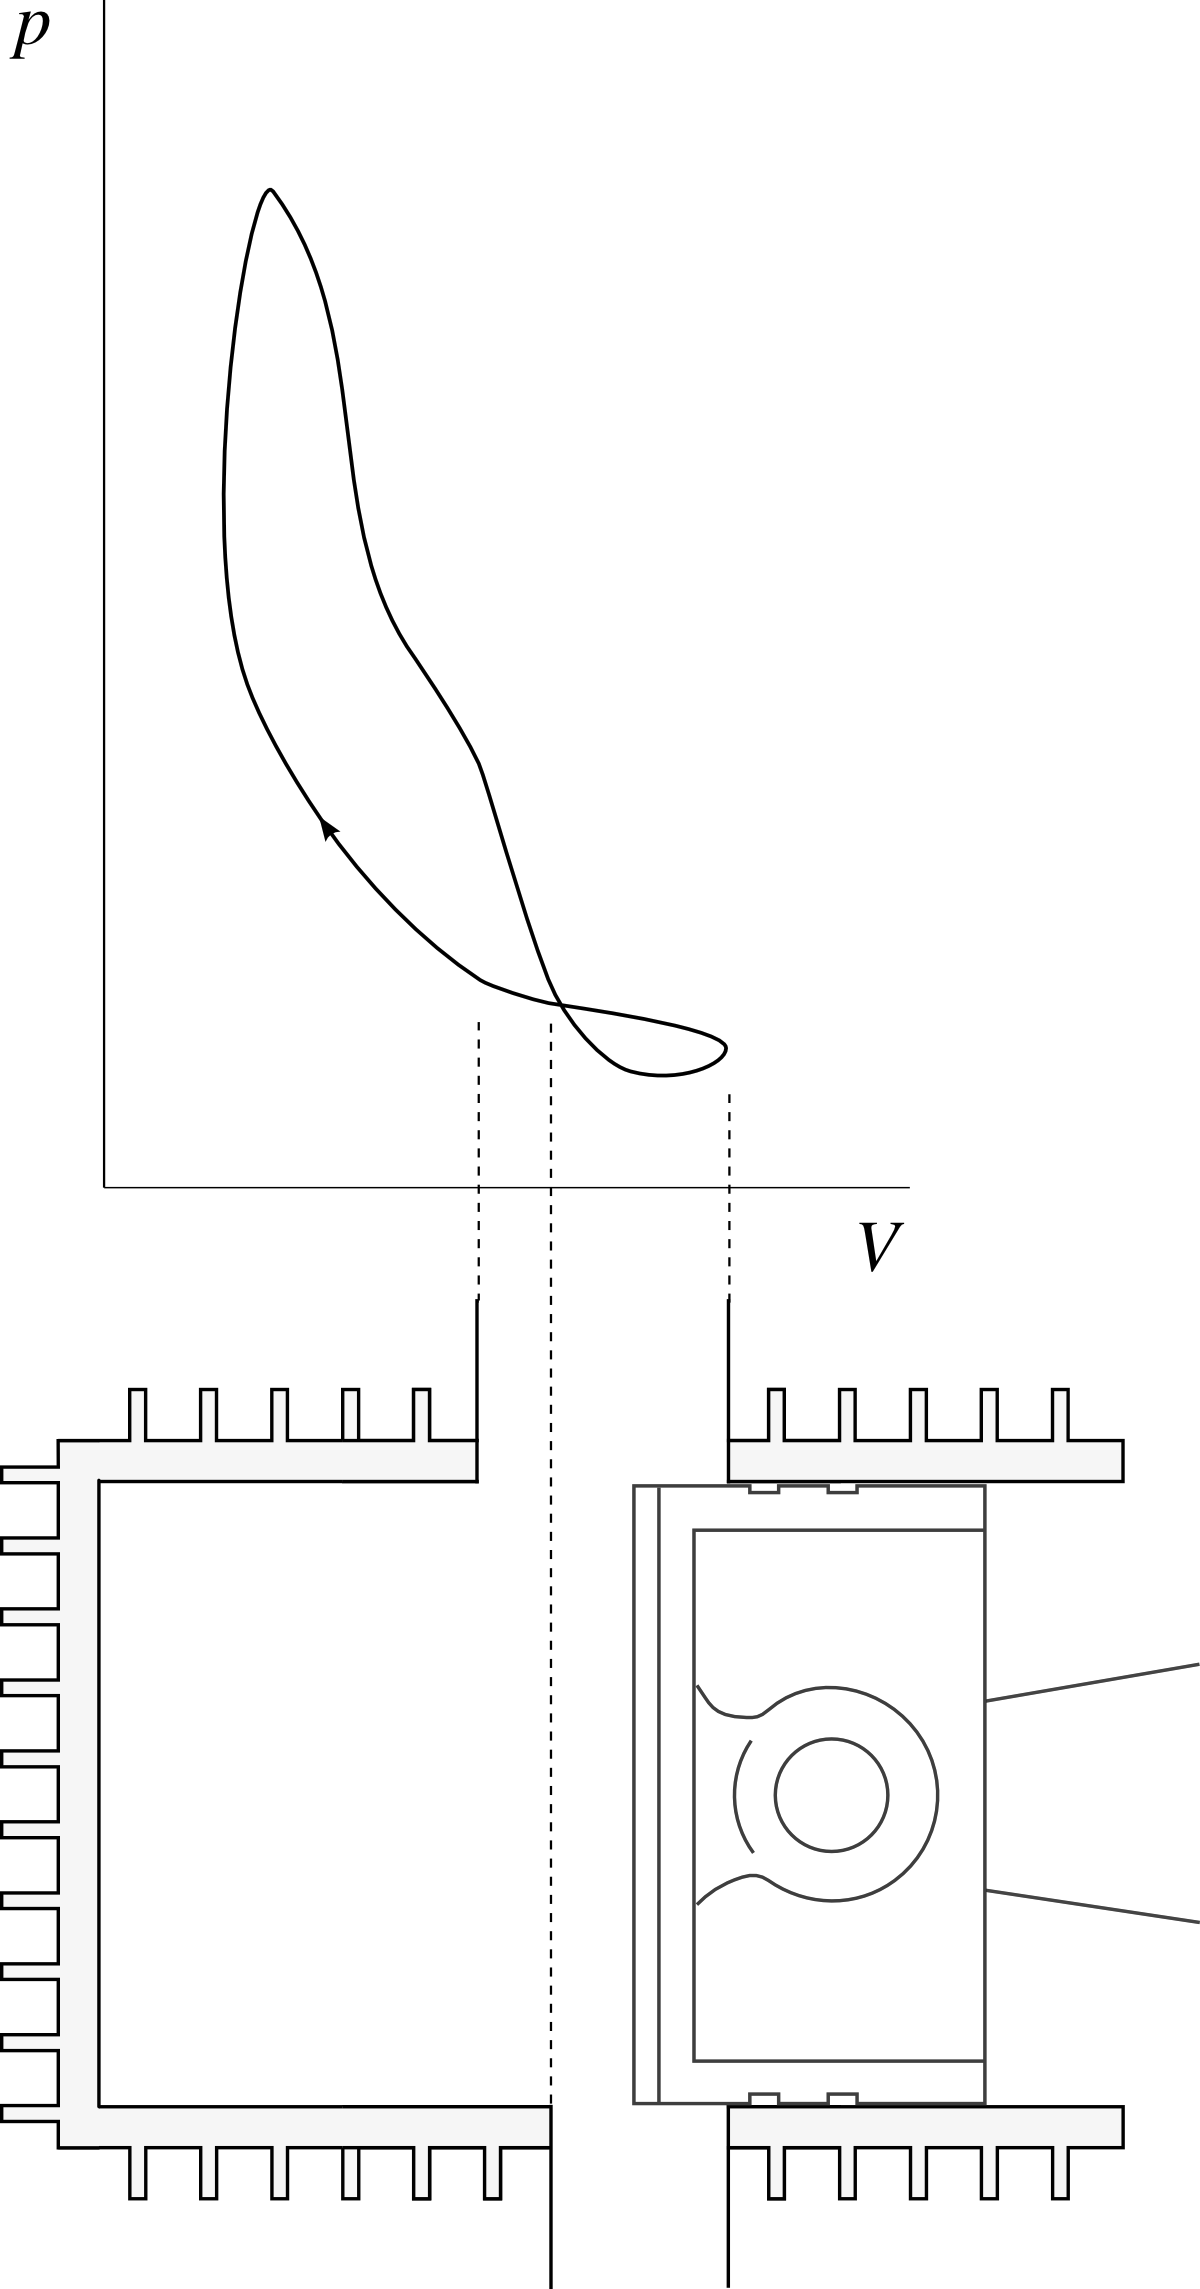
\includegraphics[width=6cm]{images/pv_deux_temps.png}
			\supercaption{Diagramme pression-volume schématique du cylindre d’un moteur deux-temps à admission carter. Il est laissé à l’étudiant/e le loisir de retrouver laquelle des deux lumières (haute ou basse) correspond à l’admission et à l’échappement dans le cylindre.}%
			{schéma dérivé d’\wcfile{Motor 2 timpi.png}{un schéma} \ccbysa par \wcu{Terraflorin}}
			\label{fig_pv_deux_temps}
		\end{center}
	\end{figure}
	
	\index{Kaaden, Walter}
	Le développement du moteur à deux temps est conjoint à celui du moteur quatre-temps, mais son développement connaîtra son plus grand essor après la seconde guerre mondiale. Le perfectionnement par l’ingénieur allemand \we{Walter Kaaden} d’un ingénieux système d’échappement, dont la seule géométrie augmente le débit d’air s’échappant pendant les détentes et le réduit lors des compressions, rend alors le moteur très compétitif sur les motos de course ; ce \vocab{pot de détente accordé} (\cref{fig_pot_detente_accorde}) sera adopté sur de nombreux modèles de production. 	
	
	\begin{figure}
		\begin{center}
			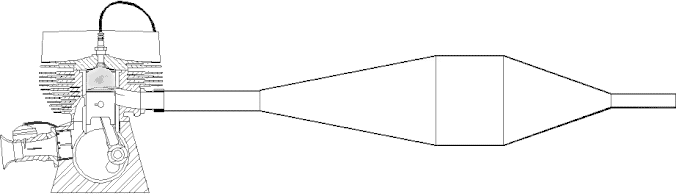
\includegraphics[width=\textwidth]{images/pot_detente_accorde.png}
			\supercaption{Pot de détente accordé (parfois dit "harmonique") monté sur un moteur deux-temps. Comme l’écoulement est instationnaire, il est possible de jouer sur la pression qu’exercent les quantités fixes de gaz rejetés sur la lumière d’échappement lorsqu’ils traversent le pot. La traversée de la partie expansive réduit la pression (et facilite donc la vidange pendant la descente du piston), tandis que le passage dans le rétrécissement, au contraire, augmente cette pression (et réduit donc les pertes de gaz pendant la remontée du piston).}%
			{\wcfile{Arbeitsweise Zweitakt.gif}{schéma} \ccbysa par Achim Agster}
			\label{fig_pot_detente_accorde}
		\end{center}
	\end{figure}
	
	\index{Day, Joseph}
	En parallèle, les idées formulées par l’entrepreneur anglais \we{Joseph Day} à la fin du \textsc{xix}\ieme siècle sur le mécanisme contrôlant l’admission se diffusent très largement. Avec son astucieuse \vocab{admission par carter}, c’est le piston lui-même qui sert de valve (\cref{fig_admission_carter}). L’air d’admission passe tout d’abord par le carter où tourne le vilebrequin, puis il est légèrement comprimé par le mouvement du piston pendant la détente avant de pouvoir entrer dans le cylindre. Le moteur fonctionne ainsi sans aucune soupape mobile ; la lubrification peut même être assurée simplement par injection d’huile directement dans l’air d’admission.
	
	\begin{figure}
		\begin{center}
			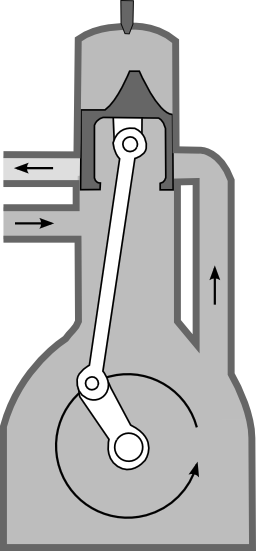
\includegraphics[width=4cm]{images/admission_carter.png}
			\supercaption{Système d’admission par carter. L’air d’admission, chargé de carburant destiné à la combustion et d’huile destinée à lubrifier les pièces mécaniques, pénètre d’abord dans le carter du vilebrequin. Il est comprimé puis inséré dans le cylindre avec le seul mouvement descendant du piston. Il n’y a besoin d’aucune valve ou soupape.}%
			{\wcfile{Silnik dwusuwowy.svg}{schéma} \pd par \wcu{Tomeq183}}
			\label{fig_admission_carter}
		\end{center}
	\end{figure}

	Avec ces deux atouts, le moteur trouve son application partout où les contraintes de poids, de volume, de coût d’acquisition et de maintenance priment sur l’efficacité. Après avoir propulsé trois millions de \textit{Trabant} en Allemagne de l’Est, il a été adopté sur la quasi-totalité des outils portatifs extérieurs (tronçonneuses, tondeuses, etc.). Le moteur se miniaturise sans difficulté, laisse de la place pour les jambes à bord d’un scooter, permet aux motoneiges de démarrer facilement, bref, jusqu’aux années~90 rien --\ pas même les associations de voisinage !\ -- ne semblait pouvoir freiner sa progression.

	\index{environnement, impact sur}\index{écologique, impact}
	Au début du \textsc{xxi}\ieme siècle, il faut pourtant renoncer à ces attraits. On peut de guerre lasse accepter le son irritant dégagé par le moteur à deux temps, mais ses émissions polluantes sont effarantes. La lubrification par injection d’huile dans l’air d’admission provoque le rejet atmosphérique de fumées, odeurs et particules nocives. En outre, la vidange toujours très incomplète du cylindre limite fortement l’efficacité de la combustion et le rendement thermique. Le durcissement des réglementations contrôlant les émissions force ainsi progressivement le remplacement de ces moteurs par d’autres à quatre temps ou par des systèmes électriques -- dont les batteries sont bien souvent chargées avec de l’énergie provenant de centrales électriques… à vapeur. On voit que des décisions technologiques a priori mineures ont parfois des conséquences à l’échelle planétaire !
	
\atendofhistorysection


\atstartofexercices
	\begin{boiboiboite}
	\propeau
	\propair
	\isentropiques
\end{boiboiboite}


\subsubsection{Efficacité d’un moteur}
\label{exo_efficacite_moteur}

	Le moteur Diesel d’une excavatrice a une efficacité de~\SI{40}{\percent} et développe une puissance continue de~\SI{60}{\kilo\watt} (c’est-à-dire environ~\SI{80}{ch}). Il est alimenté par du carburant de capacité calorifique \SI{35}{\mega\joule\per\kilogram}.
	
	\begin{enumerate}
		\item Quelle est la consommation horaire de carburant de la machine ?
		\item Quelle est la puissance qu’elle rejette sous forme de chaleur dans le conduit d’échappement ?
	\end{enumerate}

\subsubsection{Efficacité d’un réfrigérateur}
\label{exo_efficacite_refrigerateur}

	Un réfrigérateur dont le \textsc{cop} est de~\num{1,2} doit extraire \SI{100}{\kilo\joule} d’un aliment placé dans la chambre froide. Combien d’énergie électrique doit-il consommer pour cela ? Quelle quantité de chaleur aura-t-il rejetée à la fin du refroidissement ?
	

\subsubsection{Efficacité d’une pompe à chaleur}
\label{exo_efficacite_thermopompe}

	Une pompe à chaleur dont le \textsc{cop} est de~\num{3,1} fournit une puissance de~\SI{4000}{\watt} à une habitation. Quelle est la puissance électrique consommée ? Quelle est la puissance absorbée à l’atmosphère ?


\subsubsection{Thermodynamique de soirée}
\label{exo_bieres}

	Un groupe d’étudiants assoiffés par un cours de thermodynamique interminable prépare le week-end en plaçant au réfrigérateur dix packs de six bouteilles contenant une boisson à base d’eau minérale (\cref{fig_six_pack}).
	
	Une expérience effectuée sur une bouteille montre qu’elle est constituée de~\SI{172}{\gram} de verre de capacité calorifique massique \SI{0,75}{\kilo\joule\per\kilogram\per\kelvin}, et qu’elle contient \SI{25}{\centi\liter} de liquide de capacité \SI{4,2}{\kilo\joule\per\kilogram\per\kelvin}.
	
	Lorsqu’ils sont placés au réfrigérateur, les packs sont à température ambiante (\SI{19}{\degreeCelsius}). Quatre heures plus tard, ils ont atteint la température de~\SI{5}{\degreeCelsius}.
	
	\begin{figure}[htp] %handmade
		\begin{center}
		\onlyframabook{\vspace{-0.3cm}}%handmade
		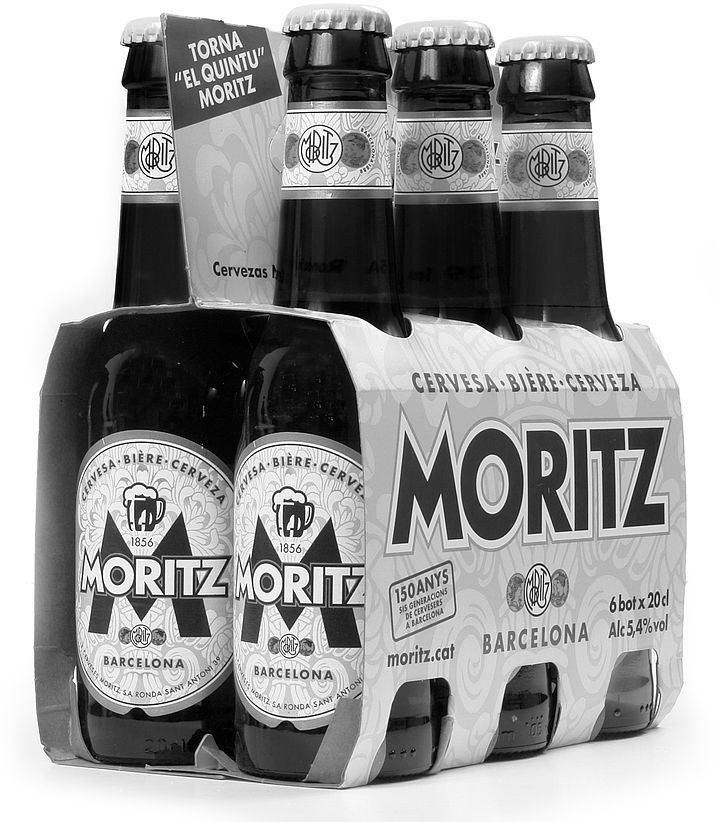
\includegraphics[width=2.5cm]{images/6-pack.jpg}
		\onlyframabook{\\\vspace{-0.6cm}}%handmade
		\end{center}
		\supercaption{Pack de six bouteilles d’un liquide utilisé pour noyer l’exaspération propre à l’étude de la thermodynamique.}{\wcfile{El_"quintu"_de_Moritz.jpg}{photo} \ccby Moritz Barcelona}
		\label{fig_six_pack}
	\end{figure}
	
	Le réfrigérateur a un rendement de~\SI{95}{\percent}. Les parois du réfrigérateur, imparfaitement isolées, absorbent de la chaleur de la pièce avec une puissance de~\SI{10}{\watt}.

	
	\begin{enumerate}
		\item Quelle quantité d’énergie électrique le réfrigérateur a-t-il consommée pendant ces quatre heures ?
	\end{enumerate}
	
	L’opérateur du réseau électrique local applique un tarif de~\SI[per-mode=symbol]{0,15}{\euroo\per\kilo\watt\per\hour}.
	
	\begin{enumerate}
		\shift{1}
		\item Quel est le coût financier du refroidissement effectué ?
		\item La pièce dans laquelle le réfrigérateur est entreposé s’est-t-elle refroidie ou réchauffée ?
		\item La pièce se refroidira-t-elle si la porte du réfrigérateur est laissée ouverte ?
	\end{enumerate}


\subsubsection{Fonctionnement d’une pompe à chaleur}
\label{exo_fonctionnement_thermopompe}

	Décrivez le cycle thermodynamique suivi par le fluide à l’intérieur d’une pompe à chaleur, en indiquant le sens des flux de chaleur et l’emplacement (intérieur/extérieur) des différents composants.
	
	Pourquoi laisse-t-on le fluide se détendre dans une soupape, au lieu d’utiliser une turbine qui pourrait fournir du travail ?
	
	\textit{On peut aussi s’exercer en s’intéressant aux cycles et configurations d’un climatiseur, d’un réfrigérateur ou d’un moteur : quelle partie est réchauffée et à quelle température ?}


\subsubsection{Algèbre}
\label{exo_algebre_rendement_climatiseur}

	Montrez, à partir de la définition du rendement du climatiseur, que celui-ci peut s’exprimer selon la relation :
			\begin{equation}
				\eta_\text{climatiseur} = \frac{1}{\left| \frac{\dot Q_\out}{\dot Q_\inn} \right| - 1} \tag{\ref{rendement_réfrigérateur_qin_qout}}
			\end{equation}
	
	\textit{Cette démonstration nous sera utile au chapitre prochain (\S\ref{ch_efficacite_maximale_machines}). On peut aussi s’exercer en s’attaquant de la même manière aux équations~\ref{eq_rendement_moteur_qin_qout} et~\ref{eq_rendement_thermopompe_qin_qout}. Attention aux valeurs absolues !}
	
	
\subsubsection{Refroidissement d’une soufflerie}
\label{exo_refrigeration_soufflerie}

	La soufflerie cryogénique \textsc{etw} (pour \textit{European Transonic Windtunnel}, \cref{fig_souffleries}) permet la circulation d’azote dans un circuit fermé pour observer les écoulements autour de maquettes. Elle permet d’atteindre Mach~\num{0,8} à~\SI{4}{\bar} et~\SI{-200}{\celsius}, à l’aide d’une soufflante de~\SI{50}{\mega\watt}.
	
	Les parois de la soufflerie sont fortement isolées, de sorte que ses transferts thermiques avec l’extérieur sont négligeables comparés aux autres transferts énergétiques. Le système de refroidissement de l’azote a un \textsc{cop} de~\num{0,8}.
	
	Lorsque la soufflerie fonctionne à plein régime, quelle puissance mécanique est consommée par le système de refroidissement ? Quelle puissance est rejetée sous forme de chaleur dans l’atmosphère ?

	\begin{figure}[htp]
		\begin{center}
			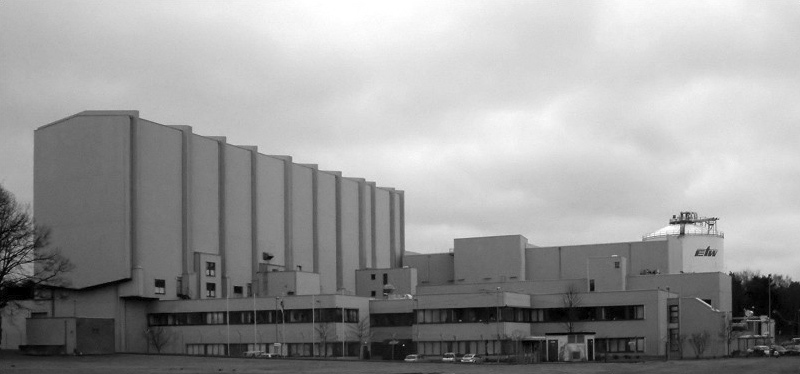
\includegraphics[width=0.8\columnwidth]{images/etw.jpg}
			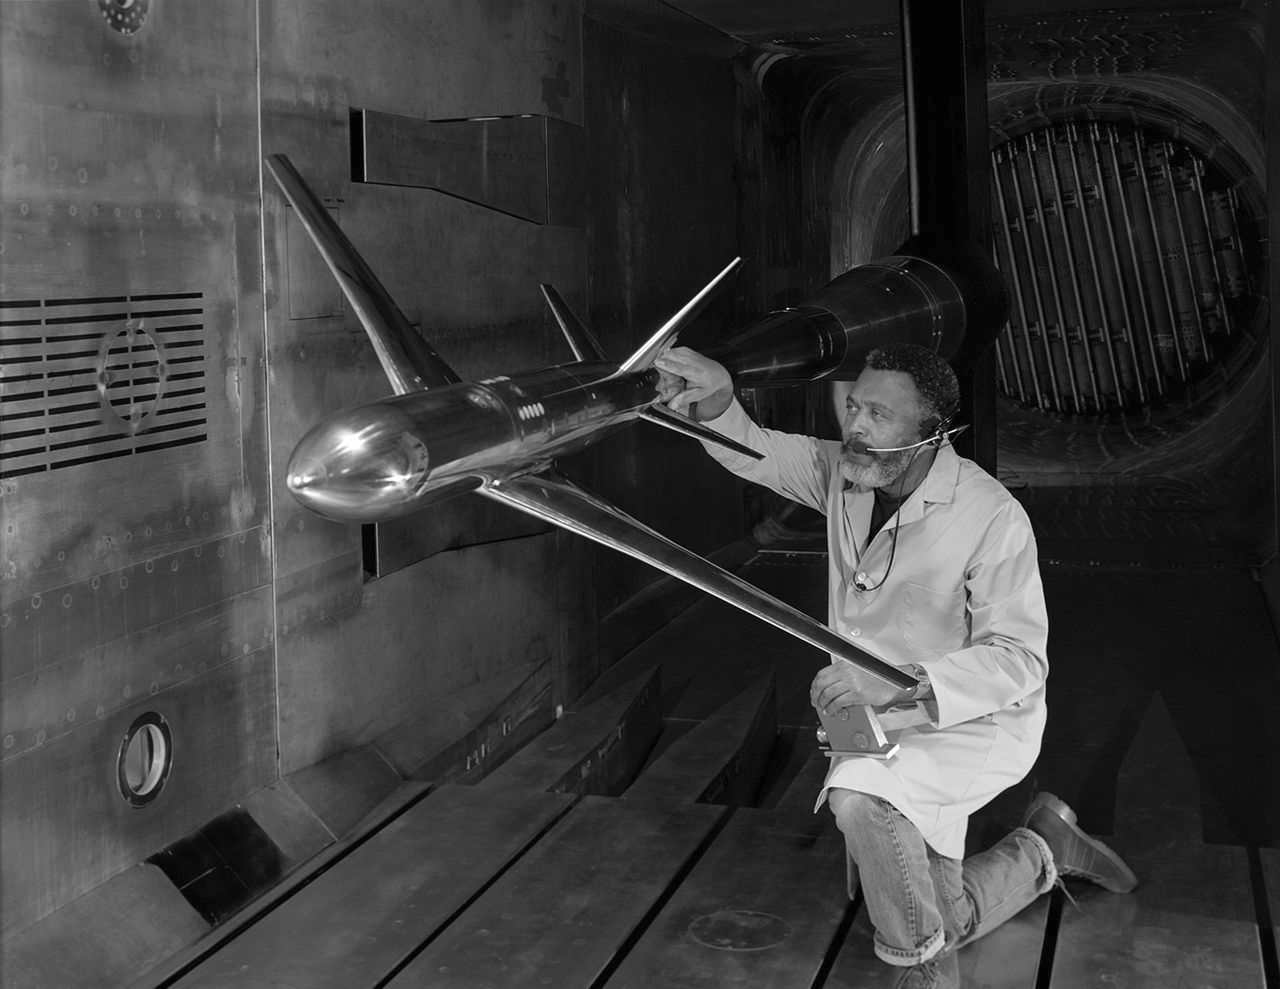
\includegraphics[width=0.8\columnwidth]{images/langley_transonic.jpg}
		\end{center}
		\supercaption{Bâtiments de l’\textsc{etw} (\textit{European Transonic Windtunnel}) à Köln et veine d’essais de la \textit{National Transonic Facility} de la \textsc{nasa}, de taille et capacités similaires.}{\wcfile{Etwrp.jpg}{Photo 1} \ccbysa par \wcu{Dantor}\\
		\wcfile{Pathfinder_I_with_Pressure_Wing_-_GPN-2000-001291.jpg}{Photo 2} \pd Fred Jones (\textsc{nasa})}
		\label{fig_souffleries}
	\end{figure}

\subsubsection{Génératrice d’électricité à turbine}
\label{exo_generatrice_electricite_turbine}

	Un turbomoteur est mis en place pour faire fonctionner une génératrice de courant électrique (\cref{fig_exo_turbomoteur}) ; il fonctionne avec un débit de~\SI{0,5}{\kilogram\per\second} d’air atmosphérique.
	
	\begin{figure}
		\begin{center}
		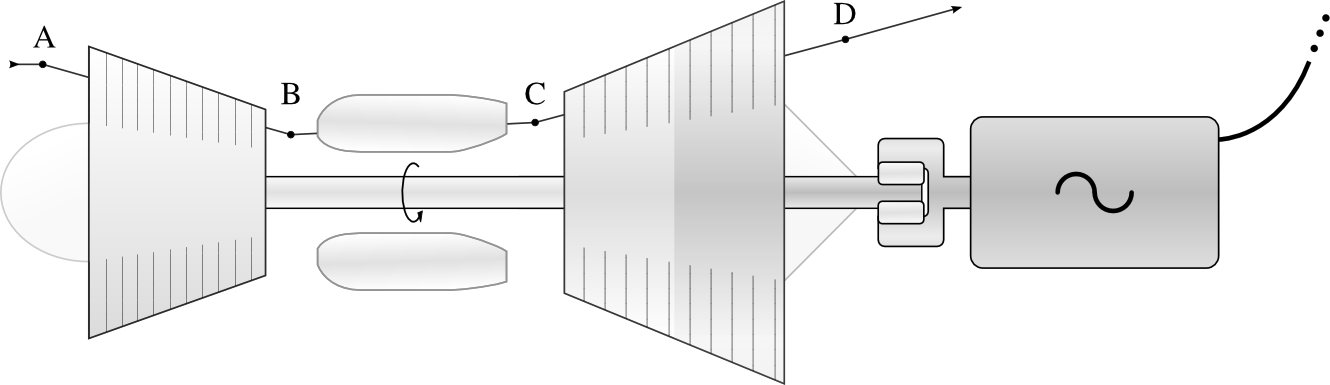
\includegraphics[width=\textwidth]{images/turbomoteur_generatrice.png}
		\end{center}
		\supercaption{Une turbomachine statique, nommée \vocab{turbomoteur}, alimentant une génératrice électrique. On tente généralement de détendre le gaz (dans la turbine, entre C et D) jusqu’à pression atmosphérique.}{schéma \ccbysa \olivier}
		\label{fig_exo_turbomoteur}
	\end{figure}
		
	\begin{itemize}
		\item L’air pénètre dans la machine à~\SI{20}{\degreeCelsius} et~\SI{1}{\bar} ; il est comprimé ($\fromatob$) jusqu’à~\SI{30}{\bar} dans le compresseur.	
		\item L’air reçoit ensuite de la chaleur par combustion, à pression constante ($\frombtoc$), jusqu’à ce que sa température atteigne \SI{1000}{\degreeCelsius}.	
		\item L’air est enfin détendu dans une turbine ($\fromctod$) jusqu’à retrouver la pression atmosphérique et être rejeté à l’extérieur.
	\end{itemize}
	
	Le compresseur est alimenté mécaniquement par la turbine et l’arbre qui les relie entraîne également la génératrice de courant.
	
	Pour étudier le rendement maximal qui pourrait être atteint par la machine, nous considérons que le compresseur et la turbine sont adiabatiques réversibles (c’est-à-dire que la compression et la détente se font de façon très lente et sans transfert de chaleur).

	\begin{enumerate}
		\item Tracez le chemin suivi par l’air pendant un cycle sur un diagramme pression-volume, de façon qualitative (c’est-à-dire sans représenter les valeurs numériques).
		\item À quelle température l’air sort-il du compresseur ?
		\item Quelle est la puissance du compresseur ?
		\item À quelle température l’air est-il rejeté dans l’atmosphère ? Quelle puissance est rejetée sous forme de chaleur dans l’atmosphère ?
		\item Quelle est l’efficacité de la machine ?
		\item Comment les quatre transferts énergétiques de cette machine théorique se comparent-ils à ceux d’une machine réelle, dans laquelle le compresseur et la turbine ne peuvent pas être réversibles ?
	\end{enumerate}


\subsubsection{Cycle d’un moteur à vapeur}
\label{exo_centrale_vapeur_cycle}

	Dans une centrale à vapeur, l’eau circule en continu en traversant quatre composants :
	
	\begin{itemize}
		\item Une pompe quasi-adiabatique dans laquelle elle rentre à l’état de liquide saturé et qui porte sa pression depuis \SI{0,5}{\bar} jusqu’à~\SI{40}{\bar} ;
		\item Une chaudière dans laquelle sa température est portée à~\SI{650}{\degreeCelsius}, à pression constante ;
		\item Une turbine quasi-adiabatique qui laisse l’eau retourner jusqu’à~\SI{0,5}{\bar} en perdant de l’énergie sous forme de travail ;
		\item Un condenseur qui refroidit l’eau à pression constante (\SI{0,5}{\bar}) jusqu’à son retour dans la pompe.
	\end{itemize}
	
	Nous acceptons les hypothèses suivantes :
		\begin{itemize}
			\item À la sortie de la turbine, la vapeur est\footnote{Après le \courshuit nous saurons prédire cette température de sortie.} à température de~\SI{110}{\degreeCelsius}.
			\item La compression dans la pompe est réversible, et la masse volumique de l’eau ne varie pas lorsqu’elle la traverse.
		\end{itemize}
	
	\begin{enumerate}
		\item Tracez le cycle suivi par l’eau sur un diagramme pression-volume et sur un diagramme température-volume, de façon qualitative.
		\item Quelle est l’efficacité du moteur ?
		\item Que se passerait-il si, pour éliminer les rejets de chaleur, on supprimait le condenseur, en connectant l’entrée de la pompe directement sur la sortie de la turbine ?
	\end{enumerate}


\subsubsection{Réfrigération industrielle}
\label{exo_refrigeration_supermache}

	Une chaîne de supermarchés fait appel à votre expertise pour évaluer la rentabilité d’un ambitieux projet de renouvellement d’une flotte de réfrigérateurs.
	
	Tous les supermarchés de l’entreprise utilisent le même modèle de réfrigérateur. Son efficacité est de~\SI{100}{\percent}.
	
	Vous vous déplacez jusqu’à un supermarché représentatif, ce qui vous permet d’effectuer des mesures et de quantifier les transferts thermiques du bâtiment. Vous mettez en évidence que :
	
	\begin{itemize}
		\item La puissance absorbée sous forme de chaleur par la chambre froide des réfrigérateurs, moyennée sur l’année, est de~\SI{80}{\kilo\watt}.
		\item L’hiver, le bâtiment perd de la chaleur avec une puissance moyenne de~\SI{400}{\kilo\watt}. Il est réchauffé avec une batterie de pompes à chaleur de \textsc{cop} \num{4}.
		\item L’été, le bâtiment absorbe de la chaleur avec une puissance moyenne de~\SI{160}{\kilo\watt}. Il est refroidi avec une batterie de climatiseurs de \textsc{cop} \num{0,9}.
		\item Pendant l’automne et le printemps, les besoins en chauffage/refroidissement sont quasi-nuls.
	\end{itemize}
	
	L’entreprise envisage de remplacer toute sa flotte de réfrigérateurs avec un modèle d’efficacité \SI{220}{\percent}, ce qui demande un investissement important. Elle compte 100 supermarchés au total, et paie l’électricité \SI{0,15}{\euroo} par~\si{\kilo\watt\hour} en moyenne.
	
	Quelle serait l’économie financière annuelle générée par le changement de modèle de réfrigérateur ?


\subsubsection{Fonctionnement d’un climatiseur}
\label{exo_fonctionnement_climatiseur}

	Un climatiseur fonctionne selon le circuit schématisé en \cref{fig_exo_climatiseur}. Le fluide utilisé dans le circuit est de l’air\footnote{On utilise souvent, en pratique, des fluides qui se liquéfient et s’évaporent dans la machine ; mais le principe de fonctionnement reste le même.}\nolinebreak.
	
	\begin{figure}
		\begin{center}
		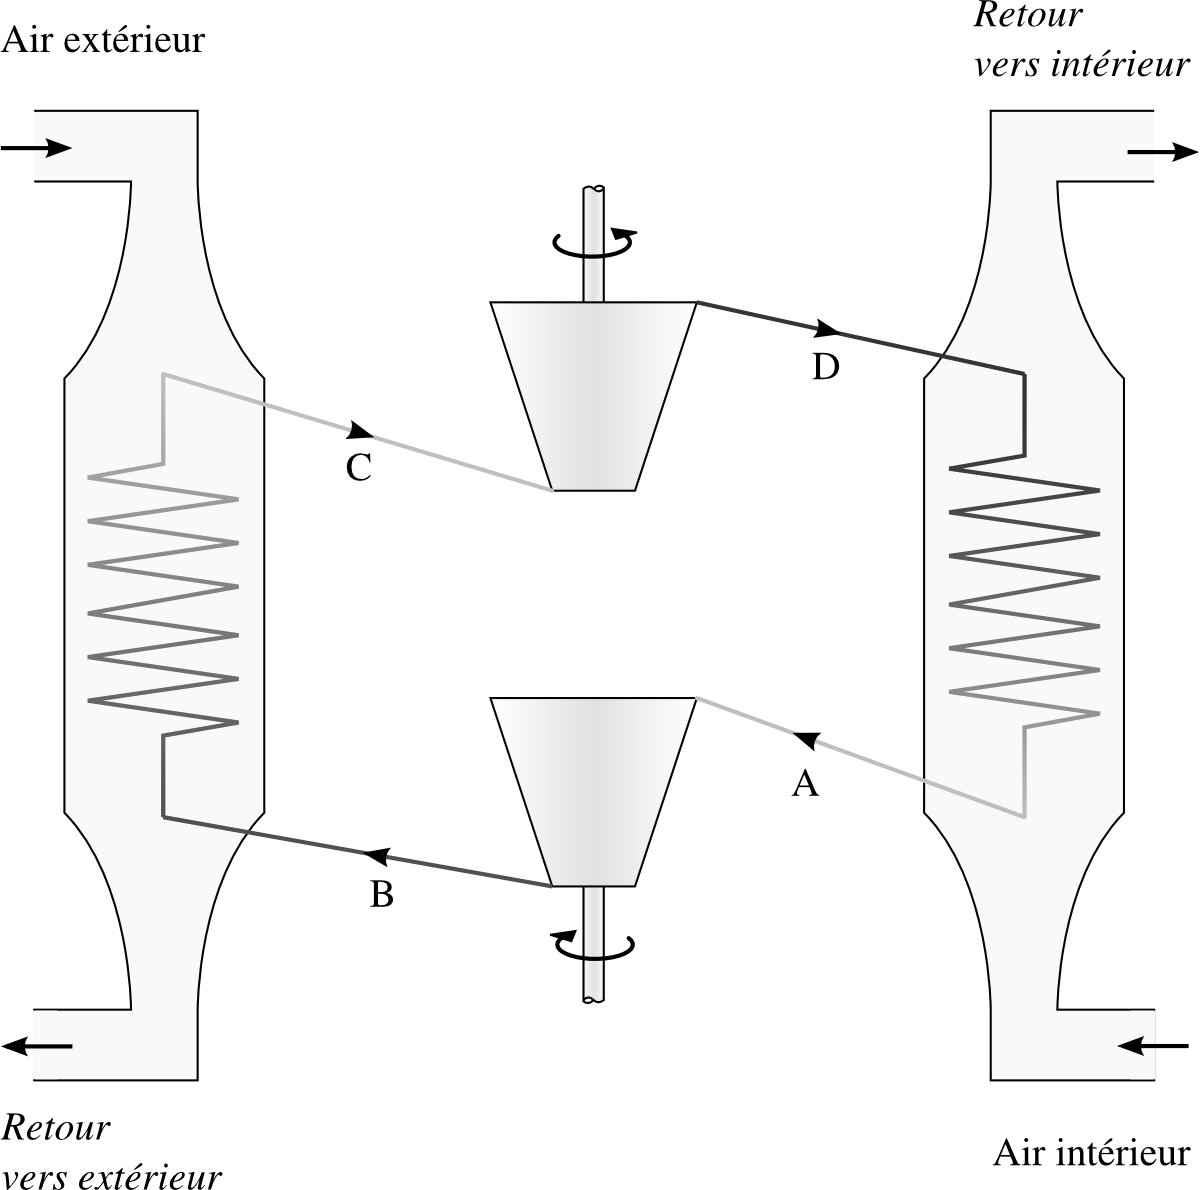
\includegraphics[width=\textwidth]{images/circuit_conditionnement_air.png}
		\end{center}
		\supercaption{Schéma de principe d’un climatiseur. L’air du circuit du climatiseur tourne en continu ($\A \to \B \to \C \to \D \to \A$), sans jamais quitter la machine.}{schéma \ccbysa \olivier}
		\label{fig_exo_climatiseur}
	\end{figure}
	
	L’air à l’intérieur du circuit y tourne de façon continue. Le compresseur et la turbine sont tous les deux adiabatiques et nous considérons qu’ils sont réversibles. Les transferts de chaleur se font à pression constante.

	Lorsqu’on met en route le climatiseur, la température extérieure et la température intérieure sont égales à~\SI{30}{\degreeCelsius}.

	Les températures de l’air à l’intérieur du circuit sont $T_\A = \SI{20}{\degreeCelsius}$, $T_\B = \SI{60}{\degreeCelsius}$, et~$T_\C = \SI{40}{\degreeCelsius}$.

	\begin{enumerate}
		\item Représentez l’évolution sur un diagramme pression-volume, de façon qualitative et en y représentant les transferts de travail et de chaleur.
		\item Quel est le rapport des pressions entre~A et~B ?
		\item Quelle est la température de l’air du circuit en~D ?
		\item Calculez les puissances spécifiques pour chacun des quatre transferts énergétiques, et calculez ainsi l’efficacité du climatiseur.
		\item Le/la propriétaire souhaite obtenir un flux d’air frais à~\SI{12}{\degreeCelsius} de débit~\SI{0,25}{\metre\cubed\per\second}. Quelle puissance électrique faut-il fournir au climatiseur pour cela ?
		\item Quel sera alors le débit minimal d’air extérieur à faire circuler dans la section extérieure du climatiseur ?
		\item Pendant l’hiver, le/la propriétaire souhaite modifier le climatiseur pour le transformer en pompe à chaleur. Décrivez (de façon qualitative) une modification du circuit pour cela, et tracez l’évolution de l’air du circuit sur un nouveau diagramme pression-volume en y indiquant les transferts énergétiques.
	\end{enumerate}


\subsubsection{Pack de conditionnement}
\label{exo_pack_conditonnement}

	Un «~pack~» de conditionnement d’air est une machine thermodynamique utilisée dans les avions de transport pour pressuriser le fuselage et pour maintenir la température dans le cockpit, la cabine et les soutes à un niveau confortable quelles que soient les conditions extérieures.
	
	Les packs (souvent appelés \textsc{ecs} ou \textsc{acm}, pour \vocabe{Environment Control System} et \vocabe{Air Cycle Machine}) sont souvent placés autour du caisson de voilure dans la zone non-pressurisée des avions de ligne (\cref{fig_pack_ssj}). Une particularité intéressante de leur fonctionnement est que c’est l’air du circuit thermodynamique lui-même qui est inséré dans la cabine à destination des passagers.
	
	\begin{figure}
		\begin{center}
			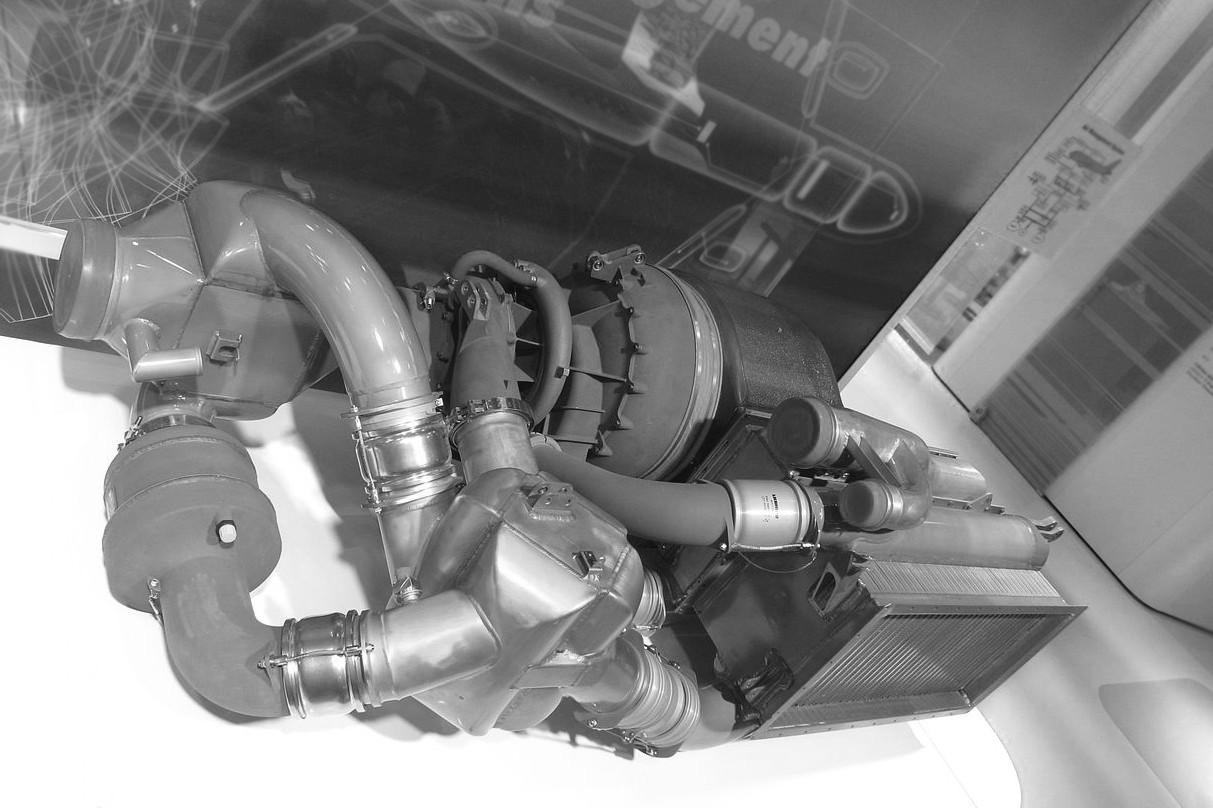
\includegraphics[height=.35\textwidth]{images/liebherr_pack.jpg}
		\end{center}
		\supercaption{Un \textsc{ecs} destiné à un \wf{Comac C919}, de longueur environ \SI{1,5}{\metre}.}{\wcfile{Air conditioning pack of Comac C919 (1).jpg}{Photo} \ccbysa \olivier}
		\label{fig_pack_c919}
	\end{figure}
	

	Nous étudions ici les fonctions de chauffage et de climatisation d’un pack : pour cela, nous simplifions la modélisation de son fonctionnement.
	
		L’air destiné à la cabine commence son chemin à l’entrée des moteurs à turbine de l’avion\footnote{Excepté lorsque l’avion, au sol, est connecté à une source d’air conditionné ou pressurisé.}. Dans le compresseur d’un de ces moteurs, sa pression est multipliée par~\num{5} pendant une évolution approximativement adiabatique et réversible ; puis il est conduit jusqu’au pack.
	
		En entrant dans le pack, cet air passe par un échangeur de chaleur où il perd de la chaleur (figure~\ref{fig_pack}). Cette chaleur est prélevée par un flux d’air distinct, dit \textsc{ram} : c’est de l’air extérieur aux conditions atmosphériques, prélevé et rejeté sous le fuselage. Les circuits d’air cabine et d’air \textsc{ram} sont à des pressions très différentes et ne sont jamais mélangés.
	
	\begin{figure}
		\begin{center}
			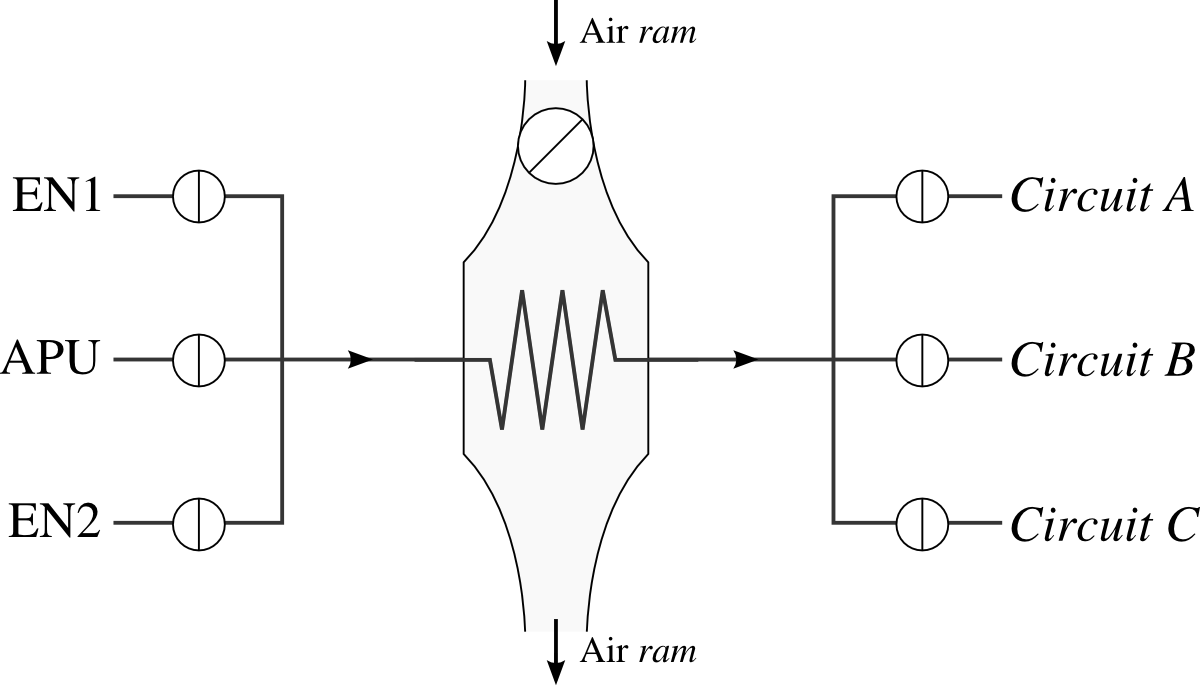
\includegraphics[width=\textwidth]{images/pack.png}
		\end{center}
		\supercaption{Circuit représentant l’air arrivant dans le pack par la gauche, en provenance des moteurs (\textsc{en1} et \textsc{en2}) ou du groupe auxiliaire de puissance (\textsc{apu}). Cet air repart dans un des trois circuits A, B ou C après avoir perdu de la chaleur au profit de l’air \textsc{ram}.}{schéma \cczero \oc}
		\label{fig_pack}
	\end{figure}

	Après son passage dans l’échangeur de chaleur, l’air du pack peut suivre trois circuits distincts avant d’arriver dans la cabine :
		\begin{description}
			\item[Le circuit A] est utilisé par temps froid, lorsque l’on souhaite porter ou maintenir la cabine à une température plus haute que la température extérieure ;
			\item[Le circuit B] est utilisé par temps modéré, lorsque la cabine doit être portée ou maintenue à température proche de la température extérieure ;
			\item [Le circuit C] est utilisé par temps chaud, lorsque les besoins en climatisation de la cabine sont importants.
		\end{description}
	
	Le pack contrôle automatiquement le débit d’air extérieur (\textsc{ram}) et sélectionne le circuit à suivre par l’air destiné à la cabine, pour porter sa température jusqu’à la valeur demandée par l’équipage au poste de pilotage (\cref{fig_320_ecs}).
	
\textbf{Circuit A : Réchauffage par temps froid}

	Dans le circuit A, l’air destiné à la cabine est simplement détendu dans une soupape (figure~\ref{fig_soupape}) avant d’être inséré dans la cabine.

	\begin{figure}
		\begin{center}
			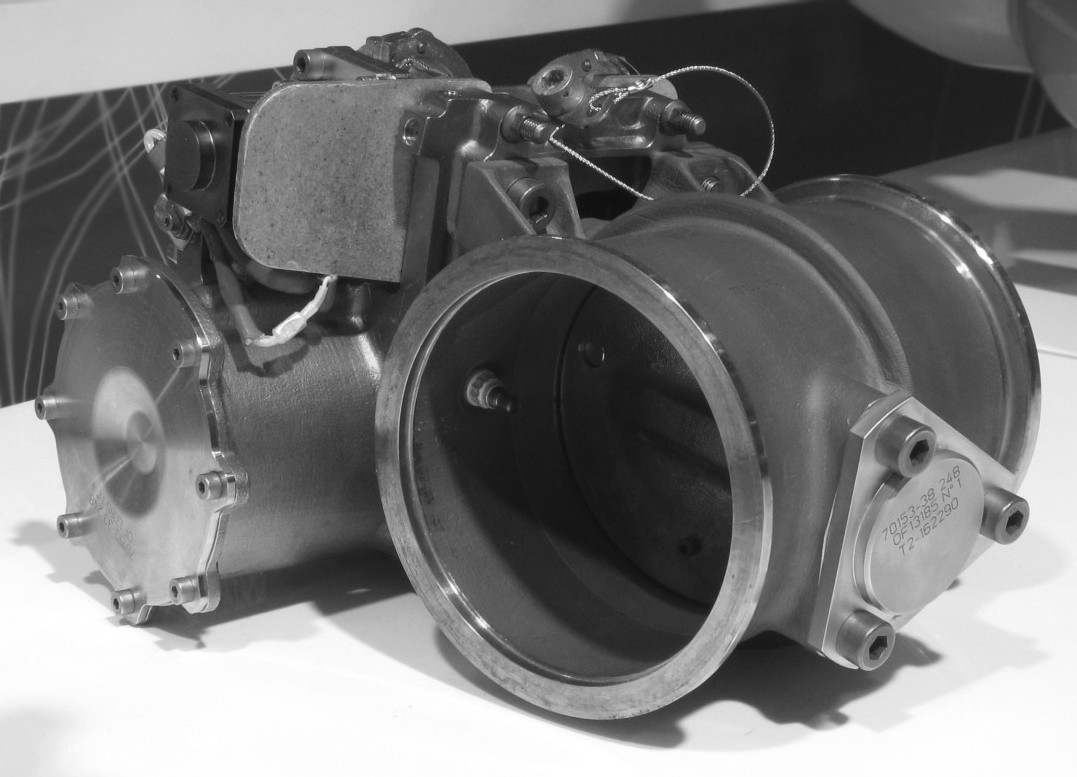
\includegraphics[height=.2\textwidth]{images/outflow_valve_1.jpg}
			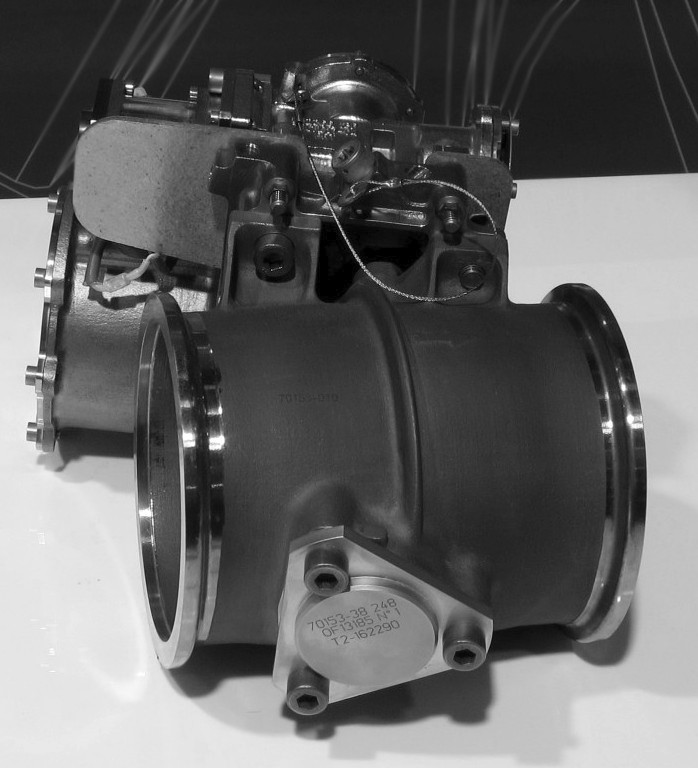
\includegraphics[height=.2\textwidth]{images/outflow_valve_2.jpg}
		\end{center}
		\supercaption{Valve de régulation de l’écoulement d’air d’un \textsc{ecs} destiné à un Comac C919.}{photos \cczero \oc}
		\label{fig_soupape}
	\end{figure}
	
	Dans la soupape, la pression chute brutalement et le volume spécifique augmente ; pourtant, aucun travail ou transfert de chaleur n’est effectué. Il s’agit d’une détente dite «~de Joule et Gay-Lussac~» (\textit{cf}. \S\ref{ch_principe_de_joule} p.\pageref{ch_principe_de_joule}). Le processus est entièrement irréversible.
	
	Lorsque l’avion est au sol par conditions climatiques froides (\SI{-35}{\degreeCelsius}, \SI{1}{\bar}) :
	
	\begin{enumerate}
		\item Quelle est la température \emph{maximale} de l’air que le pack peut insuffler en cabine ?\\
			(pour cela, nous fermerons entièrement le circuit d’air extérieur \textsc{ram}).
		\item Représentez l’évolution sur un diagramme pression-volume, de façon qualitative.
		\item Quel serait le débit minimal d’air extérieur à faire circuler dans le circuit \textsc{ram} pour amener \SI[per-mode=symbol]{0,5}{\kilogram\per\second} d’air conditionné à~\SI{24}{\degreeCelsius} dans la cabine ?
		\item Tracez l’évolution que subirait alors l’air conditionné sur le diagramme $p-v$ plus~haut.
	\end{enumerate}


	\begin{figure}
		\begin{center}
			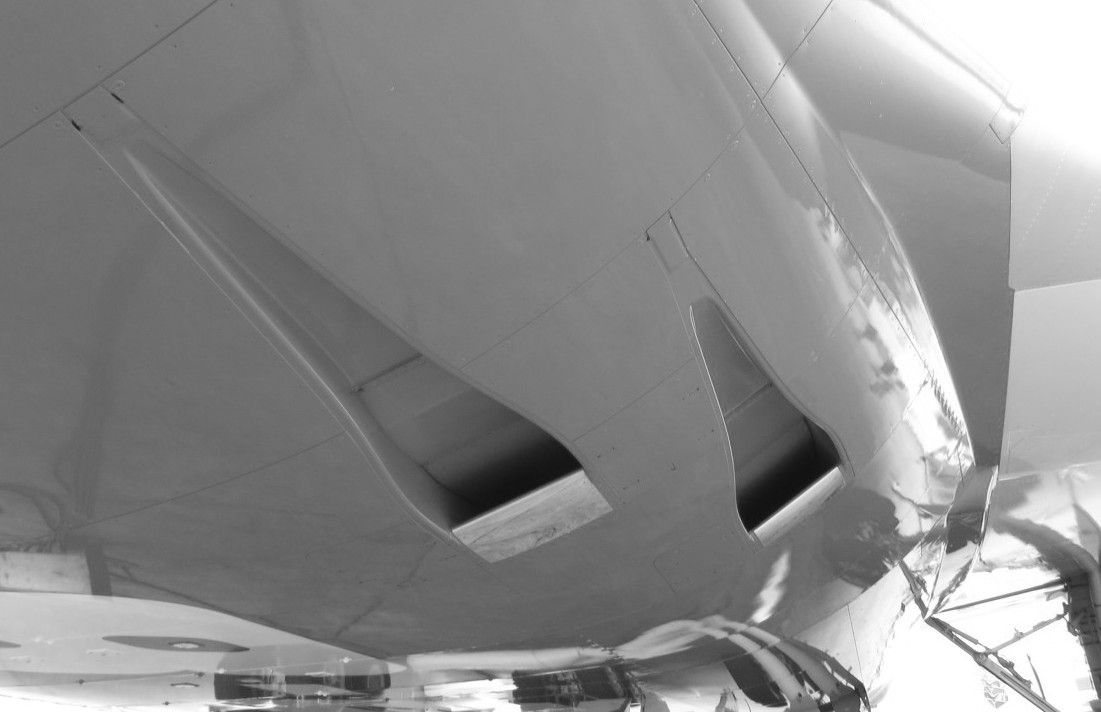
\includegraphics[height=.35\textwidth]{images/ram_pack_air_intakes_747.jpg}
		\end{center}
		\supercaption{Les entrées d’air du circuit \textsc{ram} au caisson de voilure d’un \wfd{Boeing 747-8}{Boeing 747-8I}.}{Photo \ccbysa \olivier}
		\label{fig_747_ram_intake}
	\end{figure}
	
	\begin{figure}
		\begin{center}
			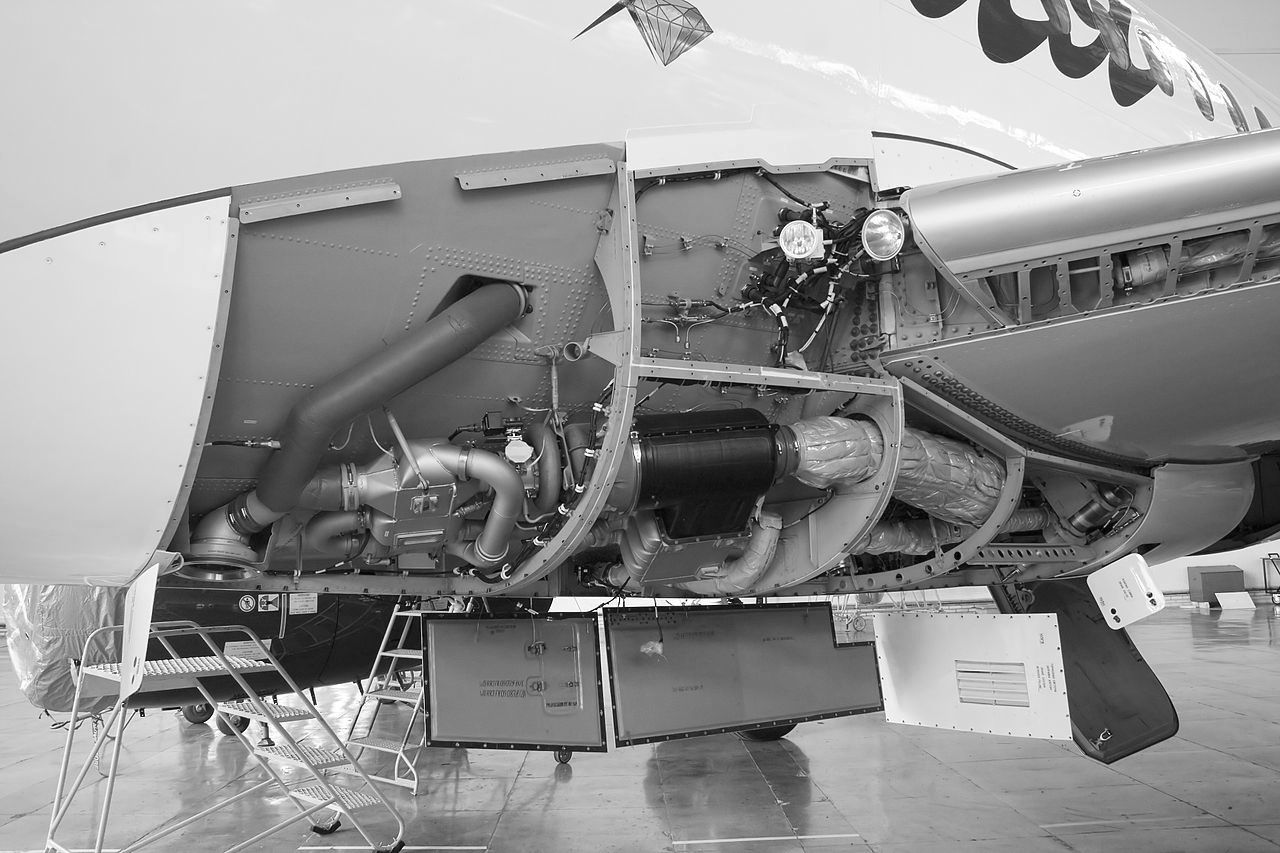
\includegraphics[width=.8\textwidth]{images/pack_sukhoi.jpg}
		\end{center}
		\supercaption{Pack de conditionnement positionné à l’emplanture d’aile d’un Sukhoi SuperJet S100}{\wcfile{Air conditioning systems of a Sukhoi Superjet.jpg}{Photo} \ccbysa A.Katranzhi}
		\label{fig_pack_ssj}
	\end{figure}


\textbf{Circuit B : Climatisation cabine par temps modéré}

	En pratique, il est possible de faire chuter la température de l’air destiné à la cabine avec un débit d’air \textsc{ram} beaucoup plus faible. Pour cette raison, lorsque les besoins en refroidissement sont importants, l’air destiné à la cabine passe par le circuit~B. Il est alors détendu à l’aide d’une turbine jusqu’à la pression cabine (\SI{1}{\bar}).  Nous considérons que la turbine est idéale (détente adiabatique réversible).
	
	Lorsque les conditions extérieures sont de~\SI{20}{\degreeCelsius}, \SI{1}{\bar} :
	
	\begin{enumerate}
	\shift{4}
		\item À quelle température l’air rentrera-t-il dans la cabine si le circuit \textsc{ram} est fermé ?
		\item Quelle énergie sera alors extraite à l’air par la turbine ?
		\item Tracez l’évolution suivie par l’air sur un diagramme pression-volume, de façon qualitative.
		\item À quelle température \emph{minimale} le circuit peut-il porter l’air destiné à la cabine ?
		\item Quelle énergie sera alors extraite à l’air par la turbine ?
		\item Tracez l’évolution sur le diagramme $p-v$ plus haut.
	\end{enumerate}

\textbf{Circuit C : Climatisation cabine par temps chaud}

	Lorsque l’appareil évolue au sol par conditions climatiques très chaudes (\SI{45}{\degreeCelsius}, \SI{1}{\bar}) l’air destiné à la cabine passe par le circuit C.
	
	Au passage dans l’échangeur, sa température ne descend que jusqu’à \SI{217}{\degreeCelsius}.
	
	Il est ensuite comprimé dans un compresseur (adiabatique réversible) jusqu’à \SI{20}{\bar}.
	
	Il passe ensuite de nouveau par un échangeur de chaleur traversé par le circuit d’air \textsc{ram}.
	
	Enfin, il est détendu dans une turbine\footnote{En pratique, il s’agit de la turbine du circuit B.} (adiabatique réversible) jusqu’à pression atmosphérique, puis insufflé dans la cabine.
		
	\begin{enumerate}
	\shift{10}
		\item Représentez le circuit suivi par l’air au travers du pack et schématisez l’évolution sur un diagramme pression-volume.
		\item À quelle température doit-on porter l’air dans le second échangeur, avant sa détente, pour obtenir un flux d’air à~\SI{5}{\degreeCelsius} dans la cabine ?
		\item Quelle est alors l’énergie sous forme mécanique que le pack reçoit ou fournit pour fonctionner ?
	\end{enumerate}

\textbf{Conclusion}
	
	\begin{enumerate}
	\shift{13}
		\item Quel est le \textsc{cop} du réchauffage généré avec le circuit A en question~3 ?
		\item Quel est le \textsc{cop} de la climatisation effectuée avec le circuit C en question~12 ?
	\end{enumerate}

	\onlyframabook{\pagebreak}
	\begin{figure}[h!]
		\begin{center}
			%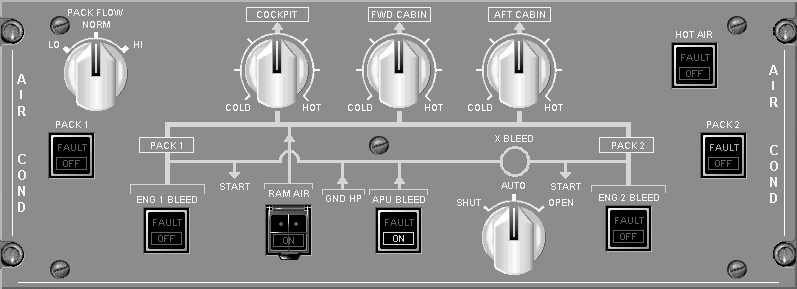
\includegraphics[width=.94\textwidth]{images/320_interface.png}
			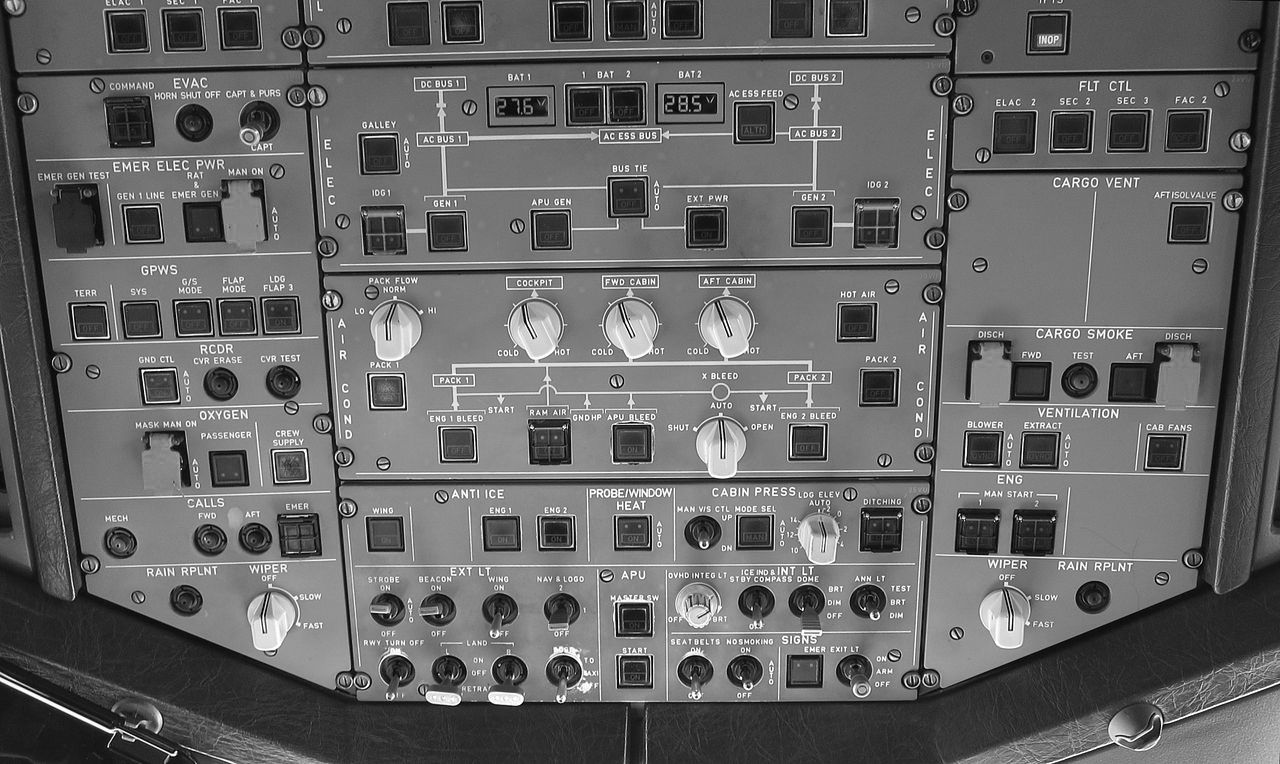
\includegraphics[width=\textwidth]{images/320_panel.jpg}
			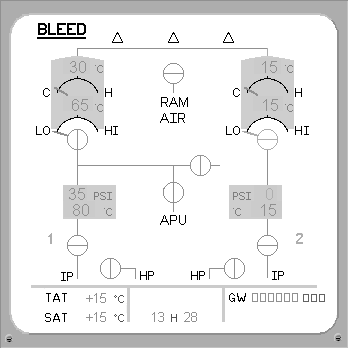
\includegraphics[width=\textwidth]{images/320_efis.png}
		\end{center}
		\supercaption{Interface de contrôle de l’\textsc{ecs} au centre du panneau supérieur du cockpit d’un Airbus A320 et le panneau d’affichage \textsc{efis} correspondant.}{\wcfile{Overhead panel of an Airbus A320 during cruise.jpg}{Photo} \ccbysa \olivier}
		\label{fig_320_ecs}
	\end{figure}	

\exercisesolutionpage
\titreresultats

\begin{description}
	\item [\ref{exo_efficacite_moteur}]
			\tab 1) $\dot Q_\inn = \frac{-\dot W_\net}{\eta_\text{moteur}} = \frac{-(\num{60e3})}{\num{0,4}} = \SI{+150}{\kilo\watt}$ ; ainsi $\dot m = \frac{\dot Q_\inn}{c_\text{carburant}} = \SI{15,4}{\kilogram\per\hour}$ (environ 12 litres par heure) ;
			\tab 2) $\dot Q_\out = -\dot Q_\inn - \dot W_\net = \SI{-90}{\kilo\watt}$.
	\item [\ref{exo_efficacite_refrigerateur}]
			\tab $W_\net = \frac{Q_\inn}{\eta_\text{réfrigérateur}} = \SI{+83,3}{\kilo\joule}$ ; $Q_\out = -Q_\inn - W_\net = \SI{-183,3}{\kilo\joule}$.
	\item [\ref{exo_efficacite_thermopompe}]
			\tab $\dot W_\net = \frac{-\dot Q_\out}{\eta_\text{thermopompe}} = \frac{-(\num{-4e3})}{\num{3,1}} = \SI{+1,29}{\kilo\watt}$ ; $\dot Q_\inn = -\dot W_\net - \dot Q_\out = \SI{+2,71}{\kilo\watt}$.
	\item [\ref{exo_bieres}]	
			\tab 1) Si l’on suppose que la masse volumique du liquide est égale à celle de l’eau liquide ($\rho_\text{liquide} = \SI{e3}{\kilogram\per\metre\cubed}$), la chaleur $Q_\inn$ absorbée par le réfrigérateur est $Q_\inn
				= - Q_\text{verre} - Q_\text{liquide} - Q_\text{parois}
				= - n_\text{bouteilles} (m_\text{verre} c_\text{verre} + m_\text{liquide} c_\text{liquide}) (\Delta T)_\text{packs} - \dot Q_\text{parois} \Delta t
				= - \num{60} (\num{0,172} \times \num{0,75e3} + \num{0,25} \times \num{4,2e3}) \times (5 - \num{19}) - \num{10} \times 4 \times \num{3600}
				= \SI{+1134,4}{\kilo\joule}$. Ainsi, $W_\net = \frac{Q_\inn}{\eta_\text{réfrigérateur}} = \SI{+1194,1}{\kilo\joule}$.
			\tab 2) $W_\net = \SI{+1194,1}{\kilo\joule} = \SI{+1194,1}{\kilo\watt\second} = \SI{+0,332}{\kilo\watt\hour}$. Ainsi le coût revient à~\SI{0,05}{\euroo} (!).
			\tab 3) La pièce sera réchauffée par le rejet $Q_\out = -Q_\inn - W_\net = \SI{-2,538}{\mega\joule}$.
			\tab 4) L’ouverture de la porte ne fait qu’augmenter la chaleur $Q_\inn$ à extraire de la chambre froide, et donc contribuera à augmenter $Q_\out$ et le réchauffement de la pièce (avec une puissance nette $\dot Q_\net = \dot Q_\inn + \dot Q_\out = -\dot W_\net$).
	\item [\ref{exo_fonctionnement_thermopompe}]
			\tab Voir \S\ref{ch_principe_fonctionnement_réfrigérateur} p.\pageref{ch_principe_fonctionnement_réfrigérateur}, et en particulier les figures~\ref{fig_refrigerateur_climatiseur_thermopompe_so}, \ref{fig_principe_du_réfrigérateur_soupape} et \ref{fig_agencement_thermopompe}.
	\item [\ref{exo_algebre_rendement_climatiseur}]
			\tab $ \eta_\text{climatiseur}
			\equiv \left|\frac{\dot Q_\inn}{\dot W_\net}\right|
			= \frac{\dot Q_\inn}{\dot W_\net}
			= \frac{\dot Q_\inn}{-\dot Q_\inn - \dot Q_\out}
			= \frac{1}{-1 - \frac{\dot Q_\out}{\dot Q_\inn}}$.
			Or, par définition $\dot Q_\out < 0$ et $\dot Q_\inn > 0$ ; ainsi $\frac{\dot Q_\out}{\dot Q_\inn} = -\left|\frac{\dot Q_\out}{\dot Q_\inn}\right|$.
			On~a donc $\eta_\text{climatiseur} = \frac{1}{-1 + \left|\frac{\dot Q_\out}{\dot Q_\inn}\right|}$. À vous maintenant avec les équations~\ref{eq_rendement_moteur_qin_qout} et~\ref{eq_rendement_thermopompe_qin_qout} !			
	\item [\ref{exo_refrigeration_soufflerie}]
			\tab Les \SI{50}{\mega\watt} dépensés par la soufflante sont entièrement dissipés sous forme de frottements dans la soufflerie, et donc convertis en chaleur qu’il faut prélever si l’on veut maintenir la température constante. Ainsi $\dot W_\net = \frac{\dot Q_\inn}{\eta_\text{réfrigération}} = \SI{+62,5}{\mega\watt}$ (un sacré réfrigérateur…). Il suit que $\dot Q_\text{out} = -\dot Q_\inn - \dot W_\net = \SI{-112,5}{\mega\watt}$.
	\item [\ref{exo_generatrice_electricite_turbine}]
			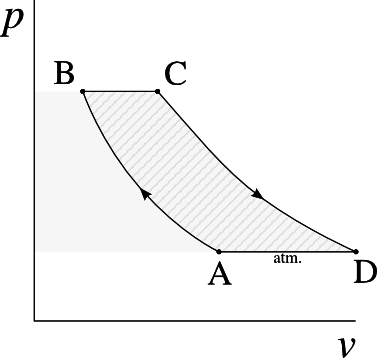
\includegraphics[height=\solutiondiagramwidth]{images/exo_sol_pv_turbomoteur_1.png}
			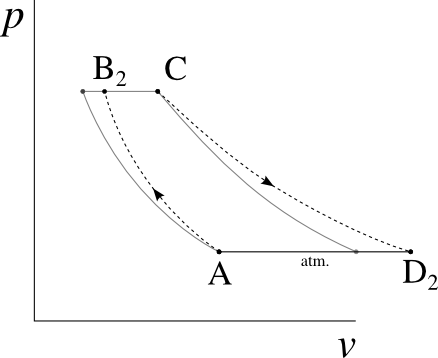
\includegraphics[height=\solutiondiagramwidth]{images/exo_sol_pv_turbomoteur_2.png}
			\tab 2) Avec l’équation~\ref{eq_isentropique_horrible2}, $T_\B = T_\A \left(\frac{p_\B}{p_\B}\right)^{\frac{\gamma - 1}{\gamma}} = \SI{774,7}{\kelvin}$ ;
			\tab 3) Avec les équations \ref{eq_grande_sfee_deltas_h} et \ref{eq_h=cpT}, $\dot W_\fromatob = \dot m c_p (T_\B - T_\A) = \SI{+242}{\kilo\watt}$  ;
			\tab 4) Avec l’équation~\ref{eq_isentropique_horrible2}, $T_\D = T_\C \left(\frac{p_\D}{p_\C}\right)^{\frac{\gamma - 1}{\gamma}} = T_\C \left(\frac{p_\B}{p_\A}\right)^{-\frac{\gamma - 1}{\gamma}} = \SI{481,8}{\kelvin}$. Ainsi, l’air rejeté doit perdre $\dot Q_\fromdtoa = c_p \Delta T = \SI{-94,8}{\kilo\watt}$ pour revenir à son état initial (\S\ref{ch_construction_cycle}) ;
			\tab 5) $\eta_\text{moteur} \equiv \left|\frac{\dot W_\net}{\dot Q_\inn} \right| = \left|\frac{\dot W_\fromatob + \dot W_\fromctod}{\dot Q_\frombtoc} \right| = \SI{62,3}{\percent} $ (fort honorable, mais seulement atteignable avec une turbine et un compresseur parfaits) ;
			\tab 6) Avec un compresseur réel $\dot W_{\fromatob_2} > \dot W_\fromatob$ et $T_{\B_2} > T_\B$.
						Il s’ensuit que si $T_\C$ est gardée constante, $\dot Q_{\frombtoc_2} < \dot Q_\frombtoc$.
						Néanmoins, on a encore $\dot W_{\fromctod_2} < \dot W_\fromctod$ et $T_{\D_2} > T_\D$ dans la turbine. La puissance $\dot W_\net$ diminue, le rejet $\dot Q_\out$ augmente. Nous montrerons au \courssept que le rendement diminue également.\\
					\textit{N.B. Nous avions déjà étudié ce moteur aux exercices \ref{exo_turbomoteur_puissances_spe} p.\pageref{exo_turbomoteur_puissances_spe} et surtout \ref{exo_generatrice_electrique} p.\pageref{exo_generatrice_electrique}. Notre capacité d’analyse et de quantification des performances s’améliore à chaque fois…}		
	\item [\ref{exo_centrale_vapeur_cycle}]
			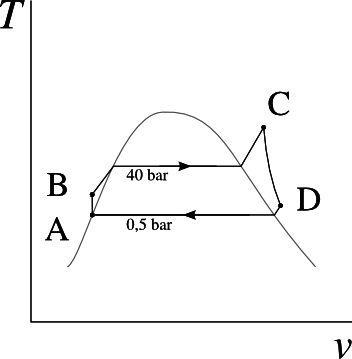
\includegraphics[height=\solutiondiagramwidth]{images/exo_sol_tv_moteur_vapeur.png}
			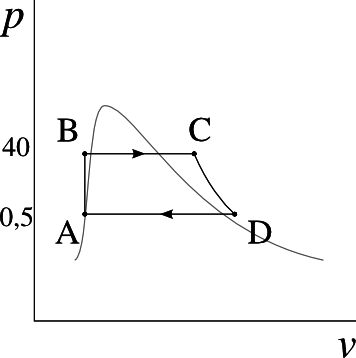
\includegraphics[height=\solutiondiagramwidth]{images/exo_sol_pv_moteur_vapeur.png}
			\tab 1) Pour s’aider à construire ces diagrammes, on peut réviser les figures~\ref{fig_t-v_eau} p.\pageref{fig_t-v_eau} et~\ref{fig_p-v_eau} p.\pageref{fig_p-v_eau}, ainsi que la section \S\ref{ch_lv_evolutions_elementaires} p.\pageref{ch_lv_evolutions_elementaires}.
			\tab 2)	$h_\A = h_{L \SI{0,5}{\bar}}$ ;
						$h_\B = h_\A + \int_\A^\B v \diff p = h_\A + v_L \Delta p $ (\ref{eq_lv_so_travail_isochore} \& \ref{eq_lv_so_chaleur_isochore} avec $q_\fromatob = 0$) ;
						$h_\C = h_{\SI{650}{\degreeCelsius} \& \SI{4}{\mega\pascal}}$ ;
						$h_\C = h_{\SI{110}{\degreeCelsius} \& \SI{0,05}{\mega\pascal}}$ ;
						Avec ces données on calcule aisément $\eta_\text{moteur} \equiv \left|\frac{w_\net}{q_\inn}\right| = -\frac{w_\net}{q_\inn} = -\frac{w_\text{turbine} + w_\text{pompe}}{q_\text{chaudière}} = -\frac{(h_\D - h_\C) + (h_\B - h_\A)}{h_\C - h_\B} = \SI{31,47}{\percent}$ (intéressant dans la mesure où on peut utiliser n’importe quel carburant).
			\tab\tab 3) Dans ce cas, la pompe ferait (presque) effectuer le chemin $\D \to \C$ à la vapeur, la ramenant à température de~\SI{650}{\degreeCelsius} et rendant impossible l’apport de chaleur dans la chaudière. Nous aurions donc effectivement une machine faite d’une turbine et d’une pompe échangeant de l’eau : impossible de dégager ainsi du travail…
	\item [\ref{exo_refrigeration_supermache}]
			\tab Dans un supermarché, au printemps comme à l’automne, l’économie d’énergie électrique permise par les nouveaux réfrigérateurs représente \SI{43,6}{\kilo\watt}.\\
			En été, la chaleur à absorber par les climatiseurs est diminuée. Il faut donc ajouter une économie de~\SI{48,5}{\kilo\watt} électriques au niveau des climatiseurs.\\
			En hiver, la chaleur à apporter par les pompes à chaleur est augmentée. Il faut donc ajouter une dépense supplémentaire de~\SI{10,9}{\kilo\watt} au niveau des pompes à chaleur.\\
			Au final, cela représente une économie annuelle de~\SI{1,672e12}{\joule} soit~\SI{69,7}{\kilo\euroo} par supermarché, qu’il faut comparer à l’investissement requis et aux coûts engendrés (notamment l’appel à votre expertise…).
	\item [\ref{exo_fonctionnement_climatiseur}]
				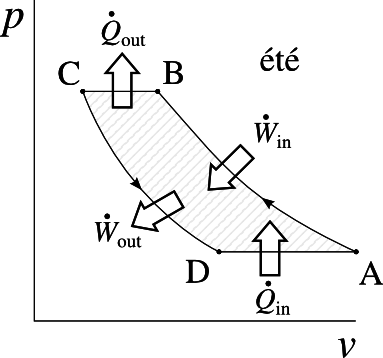
\includegraphics[height=\solutiondiagramwidth]{images/exo_sol_pv_climatiseur.png}
				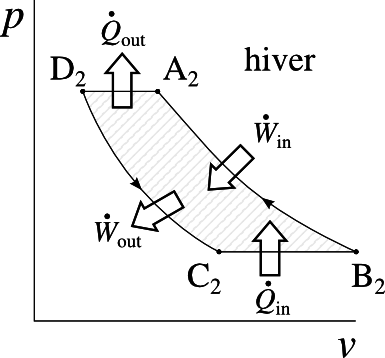
\includegraphics[height=\solutiondiagramwidth]{images/exo_sol_pv_thermopompe.png}
				\tab 2) Avec l’équation~\ref{eq_isentropique_horrible2}, $\frac{p_\B }{p_\A} = \left(\frac{T_\B}{T_\A}\right)^{\frac{\gamma}{\gamma - 1}} = \num{1,565}$ ;
				\tab 3) Idem, détente C $\to$ D adiabatique réversible, $T_\D = T_\C \left(\frac{p_\D}{p_\C}\right)^{\frac{\gamma - 1}{\gamma}} = T_\C \left(\frac{p_\A}{p_\B}\right)^{\frac{\gamma - 1}{\gamma}} = T_\C \frac{T_\A}{T_\B} = \SI{275,6}{\kelvin}$ soit \SI{2,4}{\degreeCelsius} ;
				\tab 4) Avec les équations \ref{eq_petite_sfee_deltas_h} et \ref{eq_h=cpT}, $w_\inn = \SI{+40,2}{\kilo\joule\per\kilogram}$ ;
						$q_\out = \SI{-20,1}{\kilo\joule\per\kilogram}$ ;
						$w_\out = \SI{+37,76}{\kilo\joule\per\kilogram}$ ;
						$q_\inn = \SI{+17,6}{\kilo\joule\per\kilogram}$ ;
						Ainsi avec l’\cref{def_rendement_climatiseur_refrigerateur}, $\eta_\text{climatiseur} = \num{7,213}$
				\tab 5) On veut obtenir en 2 (bouche de sortie intérieure) $\dot m_\text{air intérieur} = \frac{\dot V_2}{v_2} = \frac{\dot V_2 p_2}{R T_2} = \SI{0,305}{\kilogram\per\second}$.
						Il faut donc retirer à l’air intérieur une puissance $\dot Q_\text{air intérieur} = \dot m_\text{air intérieur} c_p (T_2 - T_1) = \SI{-5,51}{\kilo\watt}$ (\ref{eq_grande_sfee_deltas_h} \& \ref{eq_h=cpT}).
						Le climatiseur requerra donc $\dot W_\net = \frac{-\dot Q_\text{air intérieur}}{\eta_\text{climatiseur}} = \SI{765}{\watt}$.
				\tab 6) Pour minimiser $\dot m_\text{air extérieur}$, il faut maximiser sa température de sortie $T_4$. Or on a nécessairement $T_4 \leq T_\B$, sinon le transfert de chaleur se fait dans le mauvais sens. Ainsi $\dot m_\text{air extérieur min.} = \frac{-\dot Q_\text{out climatiseur}}{c_p (T_{4 \text{max.}} - T_3)} = -\frac{-\dot Q_\inn - \dot W_\net}{c_p (T_{4 \text{max.}} - T_3)} = \SI{0,208}{\kilogram\per\second}$ (minimum théorique).
				\tab\tab 7) En principe, il suffit d’inverser la position du compresseur et de la turbine. En pratique, il faudra également décaler les plages de températures pour permettre l’absorption de chaleur par temps froid.
	\item[\ref{exo_pack_conditonnement}]
			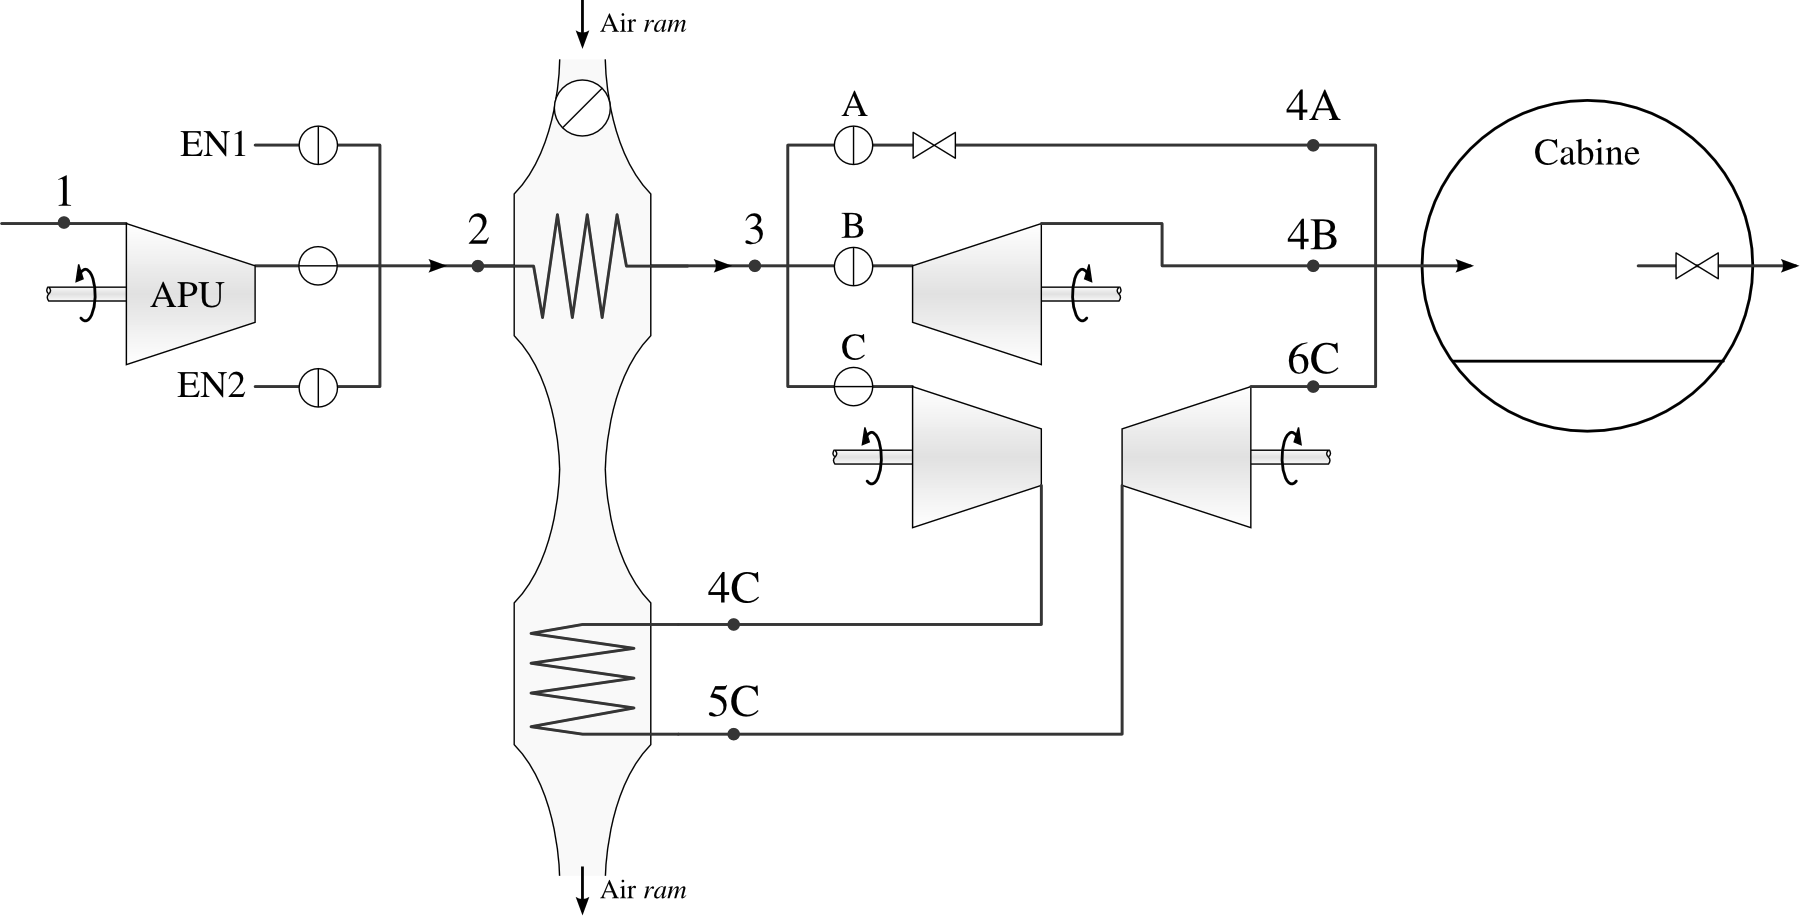
\includegraphics[width=0.9\textwidth]{images/exo_sol_circuit_acm.png}\\
			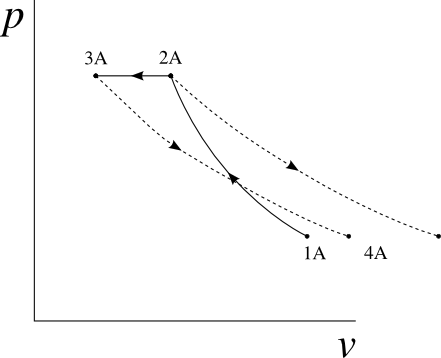
\includegraphics[height=\solutiondiagramwidth]{images/exo_sol_pv_pack_1.png}
			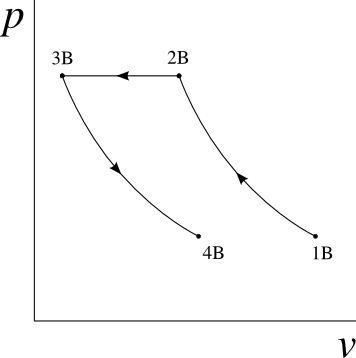
\includegraphics[height=\solutiondiagramwidth]{images/exo_sol_pv_pack_2.png}
			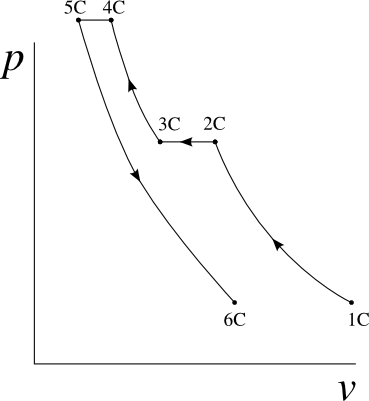
\includegraphics[width=\solutiondiagramwidth]{images/exo_sol_pv_pack_3.png}
			\tab\onlyframabook{\tab} 1) Si le circuit \textsc{ram} est fermé, alors $T_{3\A} = T_{2\A}$ ; et puisque $T_{4\A} = T_{3\A}$ (\S\ref{ch_principe_de_joule}) on obtient $T_{4\A}
			= T_{1\A} \left(\frac{p_{2\B}}{p_{1\B}}\right)^{\frac{\gamma-1}{\gamma}}
			= \SI{377,19}{\kelvin} = \SI{104,1}{\degreeCelsius}$.%handmade tabs
			\tab 3) Dans l’échangeur \textsc{ram} on a
				$\dot Q_\text{air cabine} = - \dot Q_\text{air \textsc{ram}}$ soit
				$\dot m_\text{air cabine} q_\text{air cabine} =  -\dot m_\text{air \textsc{ram}} q_\text{air \textsc{ram}}$ ou encore
				$\dot m_\text{air cabine} c_p(T_{3\A} - T_{2\A}) = -\dot m_\text{air \textsc{ram}} c_p(T_\text{rejet \textsc{ram}} - T_\text{entrée \textsc{ram}})$. Ainsi, $m_\text{air \textsc{ram}}$ est minimal lorsque $T_\text{rejet \textsc{ram}}$ est maximal, or on a nécessairement $T_\text{rejet \textsc{ram}} \leq T_{2\C}$. Ainsi,
				$\dot m_\text{air \textsc{ram} min.} = -\dot m_\text{air cabine} \frac{T_{3\A} - T_{2\A}}{T_{2\C} - T_\text{entrée \textsc{ram}}} = \SI{0,29}{\kilogram\per\second}$ (soit environ \SI{200}{\liter\per\second} à l’entrée).				
			\tab 5) Si le circuit \textsc{ram} est fermé, alors $T_{3\B} = T_{2\B}$ ; on a $T_{4\B}
			= T_{3\B} \left(\frac{p_{4\B}}{p_{3\B}}\right)^{\frac{\gamma-1}{\gamma}}
			= T_{2\B} \left(\frac{p_{1\B}}{p_{2\B}}\right)^{\frac{\gamma-1}{\gamma}}
			= T_{1\B} = \SI{293,15}{\kelvin} = \SI{20}{\degreeCelsius}$.
			\tab 6) $w_\text{turbine B} = c_p (T_{4\B} - T_{3\B}) = -w_\text{compression B} = \SI{-172}{\kilo\joule\per\kilogram}$
			\tab 8) On obtient $T_{4\B min.}$ lorsque $T_{3\B} = T_{3\B min.} = T_\text{extérieur}$. Alors $T_{4\B min.} = T_{3\B min.} \left(\frac{p_{4\B}}{p_{3\B}}\right)^{\frac{\gamma-1}{\gamma}} = \SI{185,1}{\kelvin} = \SI{-88,1}{\degreeCelsius}$ (résultat purement hypothétique bien sûr).
			\tab 9) Elle diminue : $w_\text{turbine B2} = c_p (T_{4\B min.} - T_{3\B min.}) = \SI{-108,6}{\kilo\joule\per\kilogram}$.
			\tab 12) $T_{5\C} = T_{6\C} \left(\frac{p_{5\B}}{p_{6\B}}\right)^{\frac{\gamma-1}{\gamma}} = \SI{654,6}{\kelvin} = \SI{381,5}{\degreeCelsius}$.
			\tab 13) On calcule d’abord $T_{4\C} = T_{3\C} \left(\frac{p_{4\C}}{p_{3\C}}\right)^{\frac{\gamma-1}{\gamma}} = \SI{728,4}{\kelvin}$. Dans le pack les transferts de travail sont de $w_\text{pack}
			= w_\text{compresseur pack} + w_\text{turbine pack}
			= c_p(T_{4\C} - T_{3\C}) + c_p(T_{6\C} - T_{5\C})
			= \SI{-138,9}{\kilo\joule\per\kilogram}$ ;
			Ainsi l’air dépense un travail net dans le pack, qui reçoit en permanence de l’énergie sous forme pneumatique (mécanique).
			\tab 14) Pour calculer ces \textsc{cop}, il faut compléter les cycles en faisant retourner l’air aux conditions d’entrée depuis la cabine (\S\ref{ch_construction_cycle}).
			En question~3 on a $\eta_\text{thermopompe}
			= \left|\frac{q_\out}{w_\inn}\right|
			= -\frac{c_p (T_{4\A} - T_{1\A})}{c_p (T_{2\A}-T_{1\A})}
			= \num{0,424}$ (rare application où un \textsc{cop} inférieur à~\SI{100}{\percent} est acceptable).
			\tab\tab 15) En question~12 on a $\eta_\text{climatiseur} = \left|\frac{q_\inn}{w_\inn}\right| = \frac{c_p(T_{1\C} - T_{6\C})}{c_p (T_{2\C} - T_{1\C} + T_{4\C} - T_{3\C} + T_{6\C} - T_{5\C})} = \num{0,842} $.\\
			En pratique toutefois, le travail net développé par l’air dans le pack n’est pas récupéré : il est rejeté par frottement dans l’air \textsc{ram}. On a donc $w_\net = c_p(T_{2\C} - T_{1\C})$ et le \textsc{cop} est diminué.
			\tab Quelques commentaires de fin : 1) En réalité les évolutions adiabatiques ne sont pas réversibles, ce qui réduit plus encore les rendements calculés ici. 2) Les faibles valeurs de ces rendements découlent des compromis effectués pour réduire l’encombrement, la complexité et surtout le poids des systèmes embarqués. Dans cette application, la puissance mécanique disponible est élevée, l’énergie pneumatique est largement disponible, et les dépassements en volume et en poids ont des conséquences démesurées. 3) Dans les appareils les plus récents (dits \textit{plus électriques}) tels le \wfd{Boeing 787}{B787} et l’\wfd{Airbus A350 XWB}{A350}, les packs sont désormais alimentés à l’électricité, et non plus au moyen de l’air-même destiné à la cabine.
\end{description}

\atendofexercices

